% Intended LaTeX compiler: pdflatex
\documentclass[11pt]{article}
\usepackage[utf8]{inputenc}
\usepackage[T1]{fontenc}
\usepackage{graphicx}
\usepackage{longtable}
\usepackage{wrapfig}
\usepackage{rotating}
\usepackage[normalem]{ulem}
\usepackage{amsmath}
\usepackage{amssymb}
\usepackage{capt-of}
\usepackage{hyperref}
\author{Bastien ZALUGAS}
\date{}
\title{Cours \& exercices de Python}
\hypersetup{
 pdfauthor={Bastien ZALUGAS},
 pdftitle={Cours \& exercices de Python},
 pdfkeywords={},
 pdfsubject={},
 pdfcreator={Emacs 28.2 (Org mode 9.6.1)}, 
 pdflang={French}}
\begin{document}

\maketitle
\setcounter{tocdepth}{2}
\tableofcontents


\section*{Introduction}
\label{introduction}
\subsubsection*{Manuel de Python}
\label{sec:org7245587}
Tu peux télécharger le manuel de python en \href{manuel/manuel\_python.pdf}{cliquant ici}.
\subsubsection*{Présentation}
\label{sec:orgd4c025d}
\begin{itemize}
\item Prénom
\item As-tu déjà programmé ? Si oui, avec quel langage de programmation ?
\item Motivation : pourquoi t'es-tu inscrit à ce cours ?
\end{itemize}
\subsubsection*{Notions de base}
\label{sec:orgb333390}
\begin{itemize}
\item Programmation ?
\item Programme ?
\item Langage de programmation ?
\item Instruction ?
\item Compilation ?
\item Exécution ?
\item Syntaxe ?
\end{itemize}
\subsubsection*{Pourquoi Python ?}
\label{sec:org6b7f54e}
\begin{itemize}
\item Langage interprété : versatilité (le fonctionnement ne dépend pas du système d'exploitation)
\item Syntaxe simple
\item Très utilisé dans pleins de domaines différents
\end{itemize}
\subsubsection*{Fonctionnement du cours}
\label{sec:orgca61d9e}
\textbf{Les notions dont tu auras besoin dans ce cours se trouvent dans le \href{manuel/manuel\_python.pdf}{manuel de python}.} Dans chaque cours, les chapitres que tu dois lire sont indiqués au début dans la section \textbf{Manuel}. Une fois que tu as lu les chapitres demandés, tu devras faire les exercices de la section \textbf{Exercices}.

Pour quasiment chaque exercice, on te demande de créer un \textbf{nouveau programme}, c'est à dire un \textbf{nouveau fichier}. Retiens-bien ça : \textbf{Un programme = un fichier}.

Une fois les exercices d'un cours terminés, appelle le professeur pour qu'il vienne vérifier que ce que tu as fait est correct. \textbf{N'oublie pas d'essayer ton programme avant pour être sûr que tu as terminé l'exercice et qu'il n'y a pas d'erreur.}
\subsubsection*{Introduction à IDLE}
\label{sec:orgd209d30}
\begin{itemize}
\item Sauvegarder un programme (p.18 du manuel)
\item Premier programme : Crée un premier programme nommé \texttt{bonjour.py} qui affiche le texte \textbf{\og Bonjour tout le monde !\fg{}}
\end{itemize}

\section*{Chapitre 1 : Calculs et variables}
\label{chapitre1}
\subsection*{Cours 1 : Opérateurs arithmétiques}
\label{chapitre1_cours1}
\subsubsection*{Manuel}
\label{sec:orgc89b974}
\begin{itemize}
\item \textbf{\og Calculer avec Python\fg{}}, p.22-23
\item \textbf{\og Les opérateurs de Python\fg{}}, p.23
\item \textbf{\og L'ordre des opérateurs\fg{}}, p.24-25
\end{itemize}
\subsubsection*{Exercices}
\label{sec:org3bb3f5b}
\textbf{Pour chaque exercice, il faut créer un nouveau programme.}
\begin{enumerate}
\item Dans un programme nommé \texttt{cours1.py} :
\begin{itemize}
\item Affiche le résultat d'une \textbf{addition}.
\item Affiche le résultat d'une \textbf{soustraction}.
\item Affiche le résultat d'une \textbf{multiplication}.
\item Affiche le résultat d'une \textbf{division}.
\item Affiche le résultat d'un calcul utilisant \textbf{tous les opérateurs}.
\item Affiche les résultats de \textbf{deux calculs contenant les mêmes valeurs et opérateurs} mais avec et sans \textbf{parenthèses}, pour illustrer l'ordre des opérateurs et le fonctionnement des parenthèses.
\end{itemize}
\end{enumerate}

\subsection*{Cours 2 : Variables}
\label{chapitre1_cours2}
\subsubsection*{Manuel}
\label{sec:orgefde112}
\begin{itemize}
\item \textbf{\og Les variables sont comme des étiquettes\fg{}}, p.25-26
\item \textbf{\og Utiliser les variables\fg{}}, p.26-29
\end{itemize}
\subsubsection*{Exercices}
\label{sec:org2f77dd9}
\begin{enumerate}
\item Dans un programme nommé \texttt{variables.py} :
\begin{itemize}
\item Crée une variable nommée \texttt{mon\_age} égale à ton âge, puis afficher le contenu de cette variable.
\item Crée une variable nommée \texttt{annee\_actuelle} égale à l'année actuelle.
\item Affiche le résultat de \texttt{annee\_actuelle} moins \texttt{mon\_age}.
\end{itemize}
\end{enumerate}

\section*{Chapitre 2 : Chaînes, listes, tuples, dictionnaires}
\label{chapitre2}
\subsection*{Cours 3 : Chaînes de caractères 1}
\label{chapitre2_cours3}
\subsubsection*{Manuel}
\label{sec:orga512802}
\begin{itemize}
\item \textbf{\og Les chaînes\fg{}}, p.32
\item \textbf{\og Créer des chaînes\fg{}}, p.32-33
\item \textbf{\og Gérer les problèmes de chaînes\fg{}}, p.33-36
\end{itemize}
\subsubsection*{Exercices}
\label{sec:orga4cbf56}
\begin{enumerate}
\item Dans un programme nommé \texttt{prenom\_nom.py} :
\begin{itemize}
\item Crée une variable \texttt{prenom} contenant une chaîne de caractères correspondant à ton prénom.
\item Crée une variable \texttt{nom} contenant une chaîne de caractères correspondant à ton nom de famille.
\item Affiche \textbf{\og Bonjour ! Je m'appelle \fg{}} suivi du contenu de \texttt{prenom}, puis d'un espace, puis du contenu de \texttt{nom}.
\end{itemize}

\item Dans un programme nommé \texttt{multiligne.py} :
\begin{itemize}
\item Crée une variable \texttt{ma\_journee} contenant une chaîne de caractères de plusieurs lignes racontant ta journée.
\item Affiche \texttt{ma\_journee}.
\end{itemize}

\item Dans un programme nommé \texttt{guillemets.py} :
\begin{itemize}
\item Crée une variable \texttt{guillemets} qui contient la phrase \textbf{C'est vraiment compliqué de dire \og mon prof de python est le meilleur\fg{} sans provoquer d'erreur.}.
\item Affiche cette variable.
\end{itemize}
\end{enumerate}

\subsection*{Cours 4 : Chaînes de caractères 2}
\label{chapitre2_cours4}
\subsubsection*{Manuel}
\label{sec:org7925f0e}
\begin{itemize}
\item \textbf{\og Insérer des valeurs dans des chaînes\fg{}}, p.36-37
\item \textbf{\og Multiplier des chaînes\fg{}}, p.37-38
\end{itemize}
\subsubsection*{Exercices}
\label{sec:org1586dd1}
\begin{enumerate}
\item Dans un programme nommé \texttt{prenom\_nom\_mieux.py} :
\begin{itemize}
\item Crée une variable \texttt{prenom} contenant une chaîne de caractères correspondant à ton prénom.
\item Crée une variable \texttt{nom} contenant une chaîne de caractères correspondant à ton nom de famille.
\item Affiche \textbf{\og Bonjour ! Je m'appelle <prénom> <nom>\fg{}} en remplaçant <prénom> et <nom> par les variables créées plus tôt et en utilisant \texttt{\%s}.
\end{itemize}

\item Dans un programme nommé \texttt{mon\_salaire.py} :
\begin{itemize}
\item Crée une variable \texttt{pieces\_par\_jour} contenant le nombre de pièces d'or que tu gagnes par jour.
\item Crée une variable \texttt{jours\_de\_travail} contenant le nombre de jours où tu as travaillé.
\item Affiche \textbf{\og En travaillant <jours\_de\_travail> et avec un salaire quotidien de <pieces\_par\_jour>, j'ai gagné un total de <jours\_de\_travail * pieces\_par\_jour>. Je suis riche !\fg{}} en utilisant \texttt{\%s}. Il faudra bien sûr remplacer les parties entre chevrons (<\ldots{}>) par le contenu des variables.
\end{itemize}

\item Dans un programme nommé \texttt{perroquet.py} :
\begin{itemize}
\item Crée une variable \texttt{phrase} contenant la phrase de ton choix.
\item Affiche \textbf{\og Le perroquet répète : \fg{}}.
\item Affiche 10 fois la phrase contenue dans \texttt{phrase} sans te répéter.
\end{itemize}

\item Dans un programme nommé \texttt{mur\_de\_caractères.py} :
\begin{itemize}
\item Crée une variable \texttt{caractere} qui contient un caractère de ton choix. Par exemple \og \#\fg{} ou \og -\fg{} ou ce que tu veux.
\item Crée une variable \texttt{repetition} et assigne-lui un nombre entier de ton choix.
\item Affiche autant de fois ton \texttt{caractere} que le nombre dans \texttt{repetition}.
\end{itemize}
\end{enumerate}

\subsection*{Cours 5 : Listes 1}
\label{chapitre2_cours5}
\subsubsection*{Manuel}
\label{sec:org8393984}
\begin{itemize}
\item \textbf{\og Plus puissantes que les chaînes : les listes\fg{}}, p.38-41
\end{itemize}
\subsubsection*{Exercices}
\label{sec:org4fdb45a}
\begin{enumerate}
\item Dans un programme nommé \texttt{liste\_courses.py} :
\begin{itemize}
\item Crée une variable \texttt{courses} contenant une \textbf{liste} d'au moins 5 choses à acheter. Chaque élément sera une chaîne de caractères.
\item Affiche la liste de courses.
\item Affiche le 1\textsuperscript{er} élément de la liste en utilisant son indice.
\item Affiche le 3\textsuperscript{ème} élément de la liste en utilisant son indice.
\item Modifie le 2\textsuperscript{ème} élément de la liste et l'afficher après modification.
\item Modifie le dernier élément de la liste et l'afficher après modification.
\item Affiche d'un seul coup le sous-ensemble de la liste contenant les 2\textsuperscript{ème}, 3\textsuperscript{ème} et 4\textsuperscript{ème} éléments de la liste.
\end{itemize}

\item Dans un programme nommé \texttt{liste\_courses\_quantite.py} :
\begin{itemize}
\item Crée une variable \texttt{courses\_quantite} contenant une \textbf{liste} d'au moins 5 chiffres. Après chaque chiffre, place une chaîne de caractères correspondant à quelque chose à acheter.
\item Affiche \texttt{courses\_quantite}.
\item Affiche le sous-ensemble contenant les 3\textsuperscript{ème} et 4\textsuperscript{ème} éléments de la liste.
\end{itemize}

\item Dans un programme nommé \texttt{cadavre\_exquis.py} :
\begin{itemize}
\item Crée une variable \texttt{debuts\_de\_phrases} contenant une \textbf{liste} de chaînes de caractères qui pourraient être des débuts de phrase. Par exemple, \og Aujourd'hui, j'ai décidé de\fg{}, ou alors \og Pour la nouvelle année, j'ai pris la décision de \fg{}.
\item Crée une variable \texttt{fins\_de\_phrases} contenant une \textbf{liste} de fins de phrases. Par exemple, \og être sage.\fg{}, \og devenir riche.\fg{}, \og ne plus manger de bonbons.\fg{}, etc.
\item Crée une \textbf{liste} \texttt{debuts\_et\_fins\_de\_phrases} contenant les deux listes précédemment créées.
\item Crée une variable \texttt{phrase\_entiere} contenant n'importe quel élément de la première liste contenue dans \texttt{debuts\_et\_fins\_de\_phrases} suivi de n'importe quel élément de la deuxième liste de \texttt{debuts\_et\_fins\_de\_phrases}.
\item Affiche la variable \texttt{phrase\_entiere} pour voir apparaître une phrase inattendue !
\end{itemize}
\end{enumerate}

\subsection*{Cours 6 : Listes 2}
\label{chapitre2_cours6}
\subsubsection*{Manuel}
\label{sec:org0dcb82d}
\begin{itemize}
\item \textbf{\og Ajouter des éléments à une liste\fg{}}, p.41-42
\item \textbf{\og Supprimer des éléments à une liste\fg{}}, p.42
\item \textbf{\og Arithmétique de liste\fg{}}, p.42-44
\end{itemize}
\subsubsection*{Exercices}
\label{sec:org85f84a5}
\begin{enumerate}
\item Dans un programme nommé \texttt{liste\_eleves.py} :
\begin{itemize}
\item Crée une variable \texttt{eleves} contenant la liste des prénoms des personnes présentes à l'atelier Python en omettant le tient.
\item Affiche la liste.
\item Ajoute ton prénom et celui du professeur dans la liste.
\item Affiche la liste modifiée.
\item Supprime le prénom du professeur.
\item Place ton prénom au début de la liste.
\item Affiche la liste finale.
\end{itemize}

\item Dans un programme nommé \texttt{encore\_plus\_de\_listes.py} :
\begin{itemize}
\item Crée une liste \texttt{liste\_1} avec au moins 3 éléments de ton choix.
\item Crée une liste \texttt{liste\_2} avec au moins 2 élements de ton choix.
\item Crée une liste \texttt{des\_listes} qui est la concaténation des deux autres.
\item Affiche la liste \texttt{des\_listes}.
\item Fais en sorte que la liste \texttt{des\_listes} ait 5 fois plus de contenu.
\item Affiche la liste \texttt{des\_listes}.
\end{itemize}
\end{enumerate}

\subsection*{Cours 7 : Tuples et dictionnaires}
\label{chapitre2_cours7}
\subsubsection*{Manuel}
\label{sec:org6d40443}
\begin{itemize}
\item \textbf{\og Tuples\fg{}}, p.45
\item \textbf{\og Dictionnaires\fg{}}, p.45-47
\end{itemize}

\subsubsection*{Indication complémentaire sur les dictionnaires}
\label{sec:org783caf7}
Comme vu dans le manuel, tu peux modifier une valeur dans un dictionnaire simplement en utilisant sa clef :
\begin{verbatim}
fortunes = {'Elon Musk': 180000000000, 'Jeff Bezos': 114000000000, 'Bill Gates': 104000000000, 'Mark Zuckerberg': 64400000000, 'Moi': 0}
print(fortunes)
fortunes['Moi'] = 100
print(fortunes)
\end{verbatim}
Résultat :
\begin{verbatim}
{'Elon Musk': 180000000000, 'Jeff Bezos': 114000000000, 'Bill Gates': 104000000000, 'Mark Zuckerberg': 64400000000, 'Moi': 0}
{'Elon Musk': 180000000000, 'Jeff Bezos': 114000000000, 'Bill Gates': 104000000000, 'Mark Zuckerberg': 64400000000, 'Moi': 100}
\end{verbatim}

Si tu veux \textbf{ajouter} un élément, c'est-à-dire une clef et un valeur, il faut faire comme si on modifiait la valeur de la nouvelle clef :
\begin{verbatim}
fortunes = {'Elon Musk': 180000000000, 'Jeff Bezos': 114000000000, 'Bill Gates': 104000000000, 'Mark Zuckerberg': 64400000000, 'Moi': 0}
print(fortunes)
fortunes['Mon chat'] = 100
print(fortunes)
\end{verbatim}
Résulat :
\begin{verbatim}
{'Elon Musk': 180000000000, 'Jeff Bezos': 114000000000, 'Bill Gates': 104000000000, 'Mark Zuckerberg': 64400000000, 'Moi': 0}
{'Elon Musk': 180000000000, 'Jeff Bezos': 114000000000, 'Bill Gates': 104000000000, 'Mark Zuckerberg': 64400000000, 'Moi': 0, 'Mon chat': 100}
\end{verbatim}
\subsubsection*{Exercices}
\label{sec:org1019d44}
\begin{enumerate}
\item Dans un programme nommé \texttt{mon\_tuple.py} :
\begin{itemize}
\item Crée un tuple \texttt{un\_tuple} avec au moins 3 éléments.
\item Affiche le tuple.
\item Modifie la première valeur du tuple.
\item Affiche le tuple modifié.
\end{itemize}

\item Dans un programme nommé \texttt{courses\_dictionnaire.py} :
\begin{itemize}
\item Crée un dictionnaire \texttt{courses} contenant 3 éléments à acheter comme clef avec comme valeur la quantité à acheter.
\item Affiche le dictionnaire.
\item Ajoute un élément que tu aurais oublié.
\item Supprime le premier élément du dictionnaire.
\item Modifie la deuxième entrée du dictionnaire.
\item Affiche le dictionnaire.
\end{itemize}
\end{enumerate}

\subsection*{Cours 8 : Input}
\label{chapitre2_cours8}
\subsubsection*{Cours}
\label{sec:orgaa97afb}
Jusqu'ici, nous avons donné à nos variables des valeurs directement dans le code python. Comment fait-on si l'on souhaite poser une question à l'utilisateur sans qu'il ait besoin de modifier le code ?

La méthode la plus simple, c'est d'utiliser la fonction \texttt{input()}. Nous utilisons déjà la fonction \texttt{print()} pour afficher du texte à l'écran mais nous verrons plus tard et en détail ce qu'est une fonction en programmation.

En anglais, \og input\fg{} signifie \og entrée\fg{}. La fonction \texttt{input()} sert à récupérer une \og entrée utilisateur\fg{}, c'est-à-dire les informations que l'utilisateur (celui qui utilise le programme) donne à l'ordinateur. Pour le moment, les informations seront seulement des caractères que l'utilisateur tapera au clavier. Lorsque nous utiliserons \texttt{input()}, l'utilisateur pourra entrer des caractères au clavier et terminer par la touche <Enter> ou <Entrée> pour terminer. Dans le programme, nous pourrons récupérer ce que l'utilisateur a entré dans une variable pour le réutiliser.

On peut utiliser la fonction \texttt{input()} en laissant les parenthèses vides. On peut aussi y placer un message explicatif destiné à l'utilisateur. Par exemple :
\begin{verbatim}
prenom = input("Entrez votre prénom : ")
print("Bonjour %s !" % prenom)
\end{verbatim}

Résultat :
\begin{center}
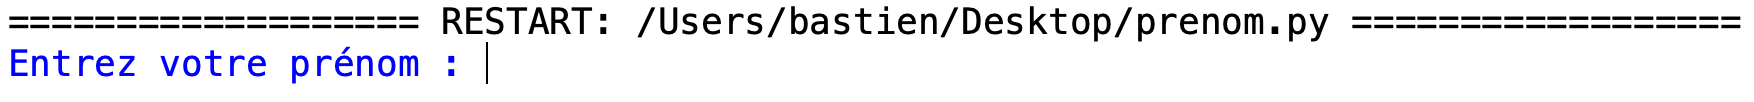
\includegraphics[width=.9\linewidth]{./img/example_prenom1.png}
\end{center}

\textbf{L'utilisateur peut entrer son prénom et appuyer sur la touche <Entrée> :}

\begin{center}
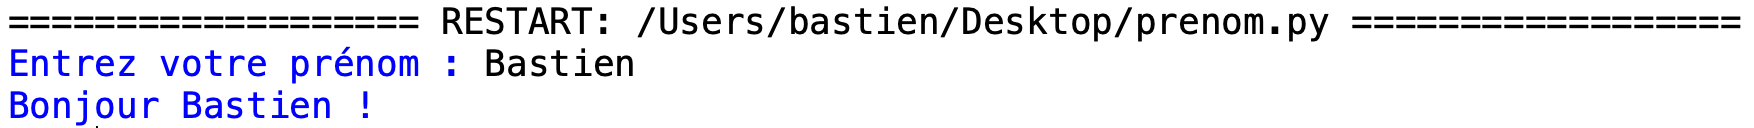
\includegraphics[width=.9\linewidth]{./img/example_prenom2.png}
\end{center}

La variable dans laquelle nous récupérons l'entrée utilisateur sera une chaîne de caractères. Si nous essayons de faire des opérations arithmétiques avec la valeur récupérée, cela va générer une erreur \og TypeError\fg{}:
\begin{verbatim}
age = input("Entrez votre âge : ")
print(age + 10)
\end{verbatim}
Résultat :
\begin{verbatim}
TypeError: can only concatenate str (not "int") to str
\end{verbatim}

Ou encore :
\begin{verbatim}
age = input("Entrez votre âge : ")
print("Tu es né en %s !" % (2022 - age))
\end{verbatim}
Résultat :
\begin{verbatim}
TypeError: unsupported operand type(s) for -: 'int' and 'str'
\end{verbatim}

Python génère une erreur car la variable \texttt{age} est une chaîne de caractères et non pas un nombre avec lequel on peut faire une opération. Pour résoudre ce problème, il nous suffit de convertir la valeur de retour de \texttt{input()} en nombre. Si nous voulons un nombre entier (sans virgule), il faut utiliser \texttt{int()}. Si nous souhaitons récupérer un nombre décimal (à virgule), nous devons utiliser \texttt{float()}.
Exemple pour convertir en un nombre entier :
\begin{verbatim}
age = int(input("Entrez votre âge : "))
print("Tu es né en %s !" % (2022 - age))
\end{verbatim}

Pour le moment, cela suffira pour créer des programmes plus intéractifs, mais nous reverrons plus en détail les conversions en python dans le chapitre 4 (cours 13).
\subsubsection*{Exercices}
\label{sec:org1b81bf4}
\begin{enumerate}
\item Dans un programme nommé \texttt{carte\_identite.py} :
\begin{itemize}
\item Pour chaque information à demander à l'utilisateur, il faudra utiliser \texttt{input()} avec une question appropriée.
\item Récupère dans une variable \texttt{prenom} le prénom de l'utilisateur.
\item Récupère dans une variable \texttt{nom} le nom de l'utilisateur.
\item Récupère dans une variable \texttt{age} l'âge de l'utilisateur.
\item Récupère dans une variable \texttt{taille} la taille de l'utilisateur.
\item Récupère dans une variable \texttt{nationalite} la nationalité de l'utilisateur.
\item Affiche \textbf{\og Je m'appelle <prenom> <nom>, j'ai <age> ans, je fais <taille>cm et mon pays d'origine est <nationalite>.\fg{}}
\end{itemize}
\end{enumerate}

\section*{Chapitre 3 : Turtle}
\label{chapitre3}
\subsection*{Cours 9 : Turtle}
\label{chapitre3_cours9}
\subsubsection*{Manuel}
\label{sec:org7ff920c}
\begin{itemize}
\item \textbf{\og Dessiner avec une tortue\fg{}}, p.49-56
\end{itemize}
\subsubsection*{Exercices}
\label{sec:orgd9ea5a3}
\begin{enumerate}
\item Dans un programme nommé \texttt{carré.py}, fais dessiner un carré à une tortue.
\item Dans un programme nommé \texttt{hexagone.py}, fais dessiner un hexagone à une tortue.
\item Dans un programme nommé \texttt{etoile.py}, fais dessiner une étoile à une tortue.
\item Dans un programme nommé \texttt{etoile\_variable.py}, fais dessiner une étoile à 5 branches à une tortue. Cependant, cette fois-ci il doit y avoir une variable nommée \texttt{taille\_cote} qui doit être utilisée pour déterminer la taille des côtés de l'étoile. Par exemple, si \texttt{taille\_cote} vaut 1, l'étoile sera composée de segments de 1 pixel de long. Si \texttt{taille\_cote} vaut 100, l'étoile sera composée de segments de 100 pixels.
\item Dans un programme nommé \texttt{visage.py}, fais dessiner un visage à une tortue. Le visage doit contenir au moins deux yeux, un nez et une bouche.
\end{enumerate}

\section*{Chapitre 4 : Les conditions}
\label{chapitre4}
\subsection*{Cours 10 : if}
\label{chapitre4_cours10}
\subsubsection*{Manuel}
\label{sec:org3def2bd}
\begin{itemize}
\item \textbf{\og Poser des questions avec if et else\fg{}}, p. 59
\item \textbf{\og Intructions if\fg{}}, p.60
\item \textbf{\og Un bloc est un groupe d'instructions\fg{}}, p.60-62
\item \textbf{\og Des conditions pour comparer des choses\fg{}}, p.62-64
\end{itemize}
\subsubsection*{Exercices}
\label{sec:orga3efe1f}
\begin{enumerate}
\item Dans un programme nommé \texttt{boutique.py} :
\begin{itemize}
\item Demande à l'utilisateur un nombre entier correspondant à la somme d'argent qu'il a et stocke sa réponse dans une variable \texttt{euros}.
\item Si \texttt{euros} est supérieure à 2, le programme doit afficher \og Tu peux t'acheter des chewing-gums\fg{} puis enlever 2 à \texttt{euros}.
\item Si \texttt{euros} est supérieure à 30, le programme devra aussi afficher \og Tu peux t'acheter des légos\fg{} puis enlever 30 à \texttt{euros}.
\item Si \texttt{euros} est supérieure à 350, le programme devra aussi afficher \og Tu peux t'acheter une playstation\fg{} puis enlever 350 à \texttt{euros}.
\item Si \texttt{euros} est supérieure à 5000000, le programme devra aussi afficher \og Tu es trop riche et tu donnes toute ta fortune !\fg{} puis \texttt{euros} devra être mise à 0.
\item Enfin, affiche \og Il te reste <euros>\fg{} en remplaçant \texttt{euros} par ce qu'il y a dans la variable.
\end{itemize}

\item Dans un programme nommé \texttt{montagnes\_russes.py} :
\begin{itemize}
\item Demande à l'utilisateur son âge puis sa taille et stocke ses réponses dans des variables \texttt{age} et \texttt{taille}.
\item Crée une condition qui affiche \og Tu es trop jeune pour faire les montagnes russes.\fg{} si \texttt{age} est strictement inférieure à 7 ans.
\item Crée une condition qui affiche \og Tu as le bon âge pour faire les montagnes russes.\fg{} si \texttt{age} est supérieure ou égale à 7 ans.
\item Crée une condition qui affiche \og Tu es trop petit pour faire les montagnes russes.\fg{} si \texttt{taille} est strictement inférieure à 60cm.
\item Crée une condition qui affiche \og Tu es trop petit pour faire les montagnes russes sans être accompagné.\fg{} si \texttt{taille} est entre 60cm inclus et 80cm exclus.
\item Crée une condition qui affiche \og Tu as la bonne taille pour faire les montagnes russes sans être accompagné.\fg{} si \texttt{taille} est supérieure ou égale à 80cm.
\end{itemize}

\item Dans un programme nommé \texttt{formes.py} :
\begin{itemize}
\item Demande à l'utilisateur un nombre entier que tu stockeras dans une variable \texttt{nb\_cotes}.
\item Demande à l'utilisateur un autre nombre entier que tu stockeras dans une variable \texttt{taille\_cote}.
\item Si \texttt{nb\_cotes} est égale à 3, une tortue doit dessiner un triangle dont les côtés sont égaux à \texttt{taille\_cote}.
\item Si \texttt{nb\_cotes} est égale à 4, une tortue doit dessiner un carré dont les côtés sont égaux à \texttt{taille\_cote}.
\item Si \texttt{nb\_cotes} est égale à 5, une tortue doit dessiner un pentagone dont les côtés doivent être égaux à \texttt{taille\_cote}.
\item Si \texttt{nb\_cotes} est strictement inférieure à 3, affiche \og Nombre de côtés trop petit.\fg{}.
\item Si \texttt{nb\_cotes} est strictement supérieure à 5, affiche \og Nombre de côtés trop grand.\fg{}.
\end{itemize}
\end{enumerate}

\subsection*{Cours 11 : if, elif, else}
\label{chapitre4_cours11}
\subsubsection*{Manuel}
\label{sec:orgdc82fcb}
\begin{itemize}
\item \textbf{\og Instructions si-alors-sinon\fg{}}, p.64-65
\item \textbf{\og Instructions if et elif\fg{}}, p.65-66
\end{itemize}
\subsubsection*{Exercices}
\label{sec:org2bc8733}
\begin{enumerate}
\item Dans un programme nommé \texttt{dragon.py} :
\begin{itemize}
\item Affiche \og Tu te trouves dans une pièce obscure d'un mystérieux château.\fg{}.
\item Affiche \og Tu dois choisir entre trois portes. Choisis 1, 2 ou 3\ldots{} \fg{} et récupère la réponse de l'utilisateur dans une variable \texttt{choix}.
\item Si le joueur a choisi la porte 1, affiche \og Tu as trouvé un trésor, tu es riche !\fg{}.
\item Si le joueur a choisi la porte 2, affiche \og La porte s'ouvre et un ogre affamé te donne un coup de massue. Perdu !\fg{}.
\item Si le joueur a choisi la porte 3, affiche \og Il y a un dragon dans cette pièce. Le dragon se réveille et te mange. Il te trouve délicieux\ldots{} Perdu !\fg{}.
\item Si le joueur a choisi autre chose, affiche \og Désolé, il faut entrer 1, 2 ou 3.\fg{}.
\end{itemize}

\item Dans un programme nommé \texttt{endroit\_secret.py} :
\begin{itemize}
\item Crée une variable \texttt{mot\_secret} égale au mot de ton choix.
\item Crée une variable \texttt{humeur\_gardien} égale à un entier entre 0 et 10.
\item Demande à l'utilisateur d'entrer son mot secret et stocke-le dans une variable \texttt{mot\_utilisateur}.
\item En utilisant \texttt{if}, \texttt{elif} et \texttt{else}, implémente les conditions suivantes :
\begin{itemize}
\item Si le \texttt{mot\_utilisateur} est égal au \texttt{mot\_secret}, affiche \og Bienvenue, vous êtes VIP !\fg{}.
\item Si le \texttt{mot\_utilisateur} est différent de \texttt{mot\_secret}, il y a 3 possibilités :
\begin{itemize}
\item Soit le gardien est de mauvaise humeur (\texttt{humeur\_gardien} inférieure à 3). Dans ce cas, affiche \og Veuillez procéder à une vérification des papiers.\fg{}.
\item Soit le gardien est de bonne humeur (\texttt{humeur\_gardien} supérieure à 7). Dans ce cas, affiche \og Bienvenue, mais vous n'êtes pas VIP.\fg{}.
\item Soit le gardien est neutre. Dans ce cas, affiche \og Veuillez prendre connaissance des règles avant d'entrer.\fg{}.
\end{itemize}
\end{itemize}
\end{itemize}
\end{enumerate}

\subsection*{Cours 12 : and, or}
\label{chapitre4_cours12}
\subsubsection*{Manuel}
\label{sec:orgaf4e743}
\begin{itemize}
\item \textbf{\og Combiner des conditions\fg{}}, p.66
\end{itemize}
\subsubsection*{Exercices}
\label{sec:orgfb2c659}
\begin{enumerate}
\item Dans un programme nommé \texttt{montagnes\_russes2.py} :
\begin{itemize}
\item Demande à l'utilisateur son âge puis sa taille et stocke ses réponses dans des variables \texttt{age} et \texttt{taille}.
\item En utilisant seulement deux \texttt{if} et en utilisant \texttt{and} et \texttt{or}, implémente les conditions suivantes :
\begin{itemize}
\item Si \texttt{age} est supérieure ou égale à 7 et \texttt{taille} est supérieure ou égale à 80, affiche \og Tu peux faire les montagnes russes.\fg{}.
\item Si \texttt{age} est inférieure à 7 ou \texttt{taille} est inférieure à 80, affiche \og Tu ne peux pas faire les montagnes russes.\fg{}.
\end{itemize}
\end{itemize}
\end{enumerate}

\subsection*{Cours 13 : Types de données et conversions}
\label{chapitre4_cours13}
\subsubsection*{Manuel}
\label{sec:orge5d637a}
\begin{itemize}
\item \textbf{\og Variables sans valeur : None\fg{}}, p.66-67
\item \textbf{\og Différence entre chaînes et nombres\fg{}}, p.67-69
\end{itemize}
\subsubsection*{Exercices}
\label{sec:org0ff742c}
\begin{enumerate}
\item Dans un programme nommé \texttt{types\_donnees.py} :
\begin{itemize}
\item Demande à l'utilisateur un nombre entier et stocke-le dans une variable \texttt{entier\_str}.
\item Demande à l'utilisateur un nombre décimal et stocke-le dans une variable \texttt{decimal\_str}.
\item Demande à l'utilisateur un mot de son choix et stocke-le dans une variable \texttt{mot}.
\item Convertis \texttt{entier\_str} en entier dans une variable \texttt{entier}.
\item Convertis \texttt{decimal\_str} en nombre décimal dans une variable \texttt{decimal}.
\item Si le nombre entier est égal à ton âge, affiche \og Bravo tu es tombé sur mon âge !\fg{}.
\item Si le nombre décimal est égal à 23.23, affiche \og Bravo tu as trouvé le nombre auquel je pensais !\fg{}.
\item Si le mot est égal à ton prénom, affiche \og Bravo tu as trouvé mon prénom !\fg{}.
\item Demande à nouveau un nombre entier à l'utilisateur et stocke-le directement sous forme de nombre entier dans une variable \texttt{entier2}.
\item Affiche le contenu de \texttt{entier2}.
\item Essaye ton programme en entrant un mot au lieu d'un nombre entier au début. Que se passe-t-il ?
\end{itemize}
\end{enumerate}

\section*{Chapitre 5 : Les boucles}
\label{chapitre5}
\subsection*{Cours 14 : Les boucles for}
\label{chapitre5_cours14}
\subsubsection*{Manuel}
\label{sec:org0544bc5}
\begin{itemize}
\item \textbf{\og Tourner en boucle\fg{}}, p.73
\item \textbf{\og Utiliser les boucles for\fg{}}, p.74-80
\end{itemize}
\subsubsection*{Exercices}
\label{sec:orge8faf60}
\begin{enumerate}
\item Dans un programme nommé \texttt{repetition.py} :
\begin{itemize}
\item Demande à l'utilisateur un nombre entier et stocke-le dans une variable \texttt{nombre}.
\item Fais une boucle \texttt{for} qui affiche \texttt{nombre} fois \og Je n'aurais plus jamais besoin de me répéter\fg{}.
\item Fais une boucle \texttt{for} qui affiche tous les nombres de 0 à \texttt{nombre} inclus.
\item Fais une boucle \texttt{for} qui affiche tous les nombres de 0 à \texttt{nombre} exclus.
\item Crée une liste \texttt{liste}.
\item Fais une boucle \texttt{for} qui demande \texttt{nombre} fois à l'utilisateur d'entrer un mot qui s'ajoutera à la liste.
\item Fais une boucle \texttt{for} qui affiche chaque élément de la liste ligne par ligne.
\end{itemize}

\item Dans un programme nommé \texttt{pairs.py} :
\begin{itemize}
\item Affiche tous les nombres pairs de 0 à 20 en utilisant une boucle \texttt{for}.
\end{itemize}

\item Dans un programme nommé \texttt{repetortue.py} :
\begin{itemize}
\item Crée deux variables : \texttt{distance} et \texttt{angle} et demande à l'utilisateur d'entrer leurs valeurs (nombres entiers uniquement).
\item Dans une boucle \texttt{for}, fais avancer la tortue de \texttt{distance} pixels et fais-la tourner de \texttt{angle} degrés.
\item Essaie différentes valeurs pour \texttt{distance} et \texttt{angle} pour voir ce qu'il se passe de différent.
\end{itemize}

\item Dans un programme nommé \texttt{cercle.py} :
\begin{itemize}
\item Fais dessiner à une tortue un cercle à l'aide d'une boucle \texttt{for}.
\end{itemize}

\item Dans un programme \texttt{spirale.py} :
\begin{itemize}
\item Fais dessiner à une tortue une spirale à l'aide d'une boucle \texttt{for}.
\end{itemize}

\item Dans un programme nommé \texttt{fibonacci.py} :
\begin{itemize}
\item Fais un programme qui calcule les 10 premiers nombres de la suite de fibonacci en utilisant une boucle \texttt{for}. La suite de Fibonacci est : 1, 1, 2, 3, 5, 8,\ldots{} Les deux premiers nombres de la suite sont toujours 1 et 1, puis ensuite chaque nombre est égal aux deux précédents.
\item (BONUS) : Fais avancer une tortue de chaque valeur de la suite de Fibonacci en la faisant tourner à chaque fois de 90°.
\end{itemize}
\end{enumerate}

\subsection*{Cours 15 : Boucles while}
\label{chapitre5_cours15}
\subsubsection*{Manuel}
\label{sec:org2ca6686}
\begin{itemize}
\item \textbf{\og Tant que nous parlons de boucles : while\fg{}}, p.81-83
\end{itemize}
\subsubsection*{Exercices}
\label{sec:org222cbaa}
\begin{enumerate}
\item Dans un programme nommé \texttt{repetition\_while.py} :
\begin{itemize}
\item Demande à l'utilisateur un nombre entier et stocke-le dans une variable \texttt{nombre}.
\item Fais une boucle \texttt{while} qui affiche \texttt{nombre} fois \og Je n'aurais plus jamais besoin de me répéter\fg{}.
\item Fais une boucle \texttt{while} qui affiche tous les nombres de 0 à \texttt{nombre} inclus.
\item Fais une boucle \texttt{while} qui affiche tous les nombres de 0 à \texttt{nombre} exclus.
\item Crée une liste \texttt{liste}.
\item Fais une boucle \texttt{while} qui demande \texttt{nombre} fois à l'utilisateur d'entrer un mot qui s'ajoutera à la liste.
\item Fais une boucle \texttt{while} qui affiche chaque élément de la liste ligne par ligne.
\end{itemize}

\item Dans un programme nommé \texttt{compte\_a\_rebours.py} :
\begin{itemize}
\item Demande à l'utilisateur un nombre entier de son choix et stocke-le dans une variable \texttt{nombre}
\item Fais une boucle \texttt{while} qui, tant que \texttt{nombre} est strictement supérieur à 0 :
\begin{itemize}
\item Affiche \texttt{nombre} - 1
\item Demande à l'utilisateur s'il veut continuer. Si l'utilisateur tape \textbf{'non'}, alors le programme s'arrête.
\item Sinon, \texttt{nombre} prend la valeur \texttt{nombre} - 1
\end{itemize}
\end{itemize}
\end{enumerate}

\section*{Chapitre 6 : Mise en pratique}
\label{chapitre6}
\subsection*{Cours 16 : Nombre secret}
\label{chapitre6_cours16}
\subsubsection*{Indication pour générer un nombre aléatoire}
\label{sec:org186af80}
Pour générer un nombre aléatoire, tu dois d'abord importer le module \texttt{random}. Il faut toujours importer les modules en début de programme pour plus de clarté :
\begin{verbatim}
import random
\end{verbatim}

Ensuite, pour générer le nombre et le stocker, tu dois utiliser la fonction \texttt{random.randint(min, max)}. \texttt{min} et \texttt{max} sont les valeurs minimale et maximale du nombre aléatoire souhaité.
\begin{verbatim}
nombre = random.randint(0, 10)
\end{verbatim}

\subsubsection*{Exercice}
\label{sec:org07900f5}
Dans un programme nommé \texttt{nombre\_secret.py} :
\begin{itemize}
\item Fais un jeu où l'ordinateur choisit un nombre aléatoire et le joueur doit le deviner.
\item Le programme doit choisir un nombre aléatoire entre 1 et 10 en utilisant la fonction vue avant.
\item Le joueur doit avoir 4 essais pour deviner le nombre.
\item Une fois qu'une partie est terminée (gagnée ou perdue), le programme doit demander à l'utilisateur s'il souhaite rejouer et relancer une partie si celui-ci répond \texttt{"oui"}.
\item Le nombre d'essai et le minimum et maximum du nombre secret doivent être stockés dans des variables au début du programme et qui doivent être utilisées au bon endroit dans le programme afin de permettre de choisir le nombre d'essai, le minimum et le maximum en changeant seulement la variable au début du programme.
\item A chaque essai, le programme doit :
\begin{itemize}
\item Dire au joueur entre combien et le minimum et maximum du nombre secret.
\item Demander au joueur un nombre.
\item Si le nombre entré par le joueur est le bon, le jeu doit féliciter le joueur.
\item Si le nombre entré est plus petit ou plus grand, le jeu doit informer le joueur et commencer un nouvel essai s'il en reste au joueur.
\item Si le nombre n'est pas le bon est qu'il s'agissait du dernier essai, le jeu doit informer le joueur qu'il a perdu.
\end{itemize}
\end{itemize}

\subsubsection*{BONUS}
\label{sec:org4491ef6}
\begin{itemize}
\item Si le joueur a gagné, le jeu doit se relancer avec une plus grande difficulté (moins d'essais, nombre secret maximum plus grand, \ldots{})
\item Si le joueur a perdu, le jeu doit baisser la difficulté ou retourner à la difficulté originale.
\item Des messages cachés qui ne s'affichent que si l'on réussit un certain niveau ou si on trouve le nombre secret du premier coup.
\end{itemize}


\section*{Chapitre 7 : Les fonctions}
\label{chapitre7}
\subsection*{Cours 17 : Fonctions}
\label{chapitre7_cours17}
\subsubsection*{Manuel}
\label{sec:org7bae705}
\begin{itemize}
\item \textbf{\og Recycler du code avec des fonctions et des modules\fg{}}, p.87-88
\item \textbf{\og Utiliser des fonctions\fg{}}, p.88-89
\item \textbf{\og Qu'est-ce qu'une fonction ?\fg{}}, p.89-90
\item \textbf{\og Variables et portée\fg{}}, p.90-92
\end{itemize}
\subsubsection*{Exercices}
\label{sec:org320af26}
\begin{enumerate}
\item Dans un programme nommé \texttt{fonctions1.py} :
\begin{itemize}
\item Définir une fonction ayant la signature \texttt{bonjour(prenom, nom)} qui doit afficher \og Bonjour <prenom> <nom> !\fg{}, en remplaçant <prenom> et <nom> par les arguments passés à la fonction.
\item Définir une fonction \texttt{somme(nombre1, nombre2)} qui retourne la somme des deux arguments.
\item Définir une fonction \texttt{minimum(nombre1, nombre2)} qui retourne le plus petit nombre entre les deux arguments.
\item Définir une fonction \texttt{puissance(nombre1, nombre2)} qui retourne \texttt{nombre1} puissance \texttt{nombre2}.
\item Définir une fonction fibonacci(n) qui retourne le n-ième nombre de la suite de Fibonacci. Exemples : \texttt{fibonacci(0)} -> \textbf{1}, \texttt{fibonacci(1)} -> \textbf{1}, \texttt{fibonacci(2)} -> \textbf{2}, \texttt{fibonacci(3)} -> \textbf{5}, etc.
\item Définir et appeler une fonction \texttt{menu()} qui :
\begin{itemize}
\item Affiche le nom de toutes les fonctions précédemment créées et demande à l'utilisateur quelle fonction il veut utiliser.
\item Si l'utilisateur entre 'bonjour' :
\begin{itemize}
\item Demande à l'utilisateur son prénom et son nom, stocke-les et appelle la fonction \texttt{bonjour(prenom, nom)} avec ce qu'a entré l'utilisateur
\end{itemize}
\item Si l'utilisateur entre 'somme', 'minimum' ou 'puissance' :
\begin{itemize}
\item Demande à l'utilisateur deux nombres et stocke-les dans des variables.
\item Appelle la fonction \texttt{somme(nombre1, nombre2)}, \texttt{minimum(nombre1, nombre2)} ou \texttt{puissance(nombre1, nombre2)} en fonction du choix de l'utilisateur.
\end{itemize}
\item Si l'utilisateur entre 'fibonacci' :
\begin{itemize}
\item Demande à l'utilisateur un nombre et appelle la fonction \texttt{fibonnaci(n)} avec celui-ci
\end{itemize}
\item Tant que l'utilisateur n'entre pas 'quitter', il faut que la fonction propose les choix à nouveau à l'utilisateur.
\end{itemize}
\end{itemize}

\item Dans un programme nommé \texttt{forme.py} :
\begin{itemize}
\item Définis une fonction \texttt{forme(nb\_cotes, taille\_cotes)} qui dessine une forme en utilisant une tortue. La forme doit avoir \texttt{nb\_cotes} en nombre de côtés et la taille doit être égale à \texttt{taille\_cotes}.
\item Appele plusieurs fois la fonction avec des arguments différents pour tout bien tester.
\end{itemize}

\item Dans un programme nommé \texttt{forme\_aleatoire.py} :
\begin{itemize}
\item Définis une fonction ayant la signature \texttt{forme\_aleatoire(tortue)}.
\item La fonction doit définir une variable \texttt{repetition} égale à un nombre aléatoire entre 50 et 200.
\item La fonction doit définir une variable \texttt{distance} égale à un nombre aléatoire entre 10 et 200.
\item Le programme doit définir une variable \texttt{angle} égale à un nombre aléatoire en 0 et 360.
\item La forme aléatoire doit être dessinée par la \texttt{tortue} passée en argument en répétant \texttt{repetition} fois le fait d'avancer de \texttt{distance} pixels et de tourner d'\texttt{angle} degrés.
\item Pour tester, appelle plusieurs fois cette fonction avec des tortues différentes.
\end{itemize}

\item Dans un programme nommé \texttt{inverse.py} :
\begin{itemize}
\item Définis une fonction ayant la signature \texttt{inverse(liste)} qui doit renvoyer la \texttt{liste} passée en argument à l'envers. Par exemple, si on lui donne la liste \texttt{[1, 5, 2, 6]} en argument, elle doit renvoyer \texttt{[6, 2, 5, 1]}.
\item Appelle la fonction plusieurs fois avec des listes différentes pour bien tester tous les cas.
\item Essaie de passer une chaîne de caractères en argument. Que se passe-t-il ?
\end{itemize}

\item Dans un programme nommé \texttt{minimum\_liste.py} :
\begin{itemize}
\item Définir une fonction ayant la signature \texttt{minimum\_liste(liste\_nombres)} qui prend une liste de nombre en paramètre et renvoie le plus petit nombre de la liste.
\item Appeler plusieurs fois la fonction avec différentes listes de nombres pour bien tester tous les cas.
\end{itemize}

\item Dans un programme nommé \texttt{tri.py} :
\begin{itemize}
\item Faire une fonction ayant la signature \texttt{tri(liste\_nombres)}.
\item Le paramètre \texttt{liste\_nombres} sera une liste de nombres.
\item La fonction doit renvoyer une liste qui contient tous les nombres de \texttt{liste\_nombres} triés dans l'ordre croissant.
\item Appeler plusieurs fois la fonction avec différentes listes de nombres pour tester tous les cas.
\end{itemize}
(BONUS)
\begin{itemize}
\item Définis une fonction \texttt{creerListe(taille)} qui crée une liste de taille \texttt{taille} en demandant à l'utilisateur chaque nombre de la liste et renvoie la liste ainsi créée.
\item Appelle la fonction \texttt{creerListe} après avoir demandé la \texttt{taille} à l'utiliateur puis utilise la liste créée dans la fonction \texttt{tri}. Affiche la liste avant et après avoir utilisé \texttt{tri}.
\end{itemize}
\end{enumerate}

\subsection*{Cours 18 : Les modules}
\label{chapitre7_cours18}
\subsubsection*{Cours}
\label{sec:org85a8648}
\textbf{Un module} sert à regrouper des fonctions, des variables et d'autres choses dans des programmes plus vastes et plus puissants. Certains modules sont intégrés dans Python lui-même, tandis que tu peux en télécharger d'autres de manière séparée. Nous en avons déjà utilisé par exemple avec \textbf{turtle} et \textbf{random}.

Pour utiliser un module, il suffit d'écrire au début du fichier \texttt{import nom\_du\_module}. Dans le cas où tu voudrais utiliser un module qui n'est pas intégré à Python, il faudra d'abord le télécharger (ou le coder !).

Maintenant, si je te disais que tu peux créer tes propres modules avec tes propres fonctions, variables, classes dedans !? Ne serait-il pas pratique de pouvoir utiliser sans avoir à la réécrire une fonction qui, par exemple, permet de demander un entier à l'utilisateur et de vérifier qu'il n'y a pas d'erreur ?

Pour créer ton propre module, il suffit de :
\begin{enumerate}
\item Créer un nouveau fichier et lui donner le nom de ton module, par exemple \texttt{mes\_fonctions.py}.
\item Écrire tes fonctions à l'intérieur du fichier, autant que tu veux. \textbf{Attention, nous voulons seulement écrire les fonctions, pas les utiliser tout de suite.}
\item Une fois le fichier enregistré, il suffit de le mettre dans le même \textbf{dossier} que le programme dans lequel tu vas l'utiliser puis de l'importer avec \texttt{import mes\_fonctions}.
\end{enumerate}

\subsubsection*{Exercices}
\label{sec:org91678e2}
Dans le chapitre suivant, nous allons mettre en pratique les modules et les fonctions ensemble en créant notre propre bibliothèque personnalisée de fonctions !

\begin{enumerate}
\item Dans un fichier nommé \texttt{mes\_fonctions.py} :
\begin{itemize}
\item Crée la fonction \texttt{demander\_int(message)} qui :
\begin{itemize}
\item demande un entier à l'utilisateur en affichant le message \texttt{message}.
\item retourne l'entier convertit en \texttt{int}.
\end{itemize}
\item Crée la fonction \texttt{demander\_float(message)} qui fonctionne comme la précédente mais avec un \texttt{float}.
\item Crée la fonction \texttt{demander(message)} qui fonctionne comme les précédentes mais avec une chaîne de caractères.
\end{itemize}

\item Dans un programme nommé \texttt{tests\_fonctions.py} :
\begin{itemize}
\item importe ton module \texttt{mes\_fonctions}
\item teste les 3 fonctions présentes dans ton module
\end{itemize}
\end{enumerate}

Tu as maintenant créé les 3 premières fonctions de ton propre module, que tu pourras réutiliser chaque fois que tu en as besoin. Tu es libre d'y ajouter les fonctions qui te semblent intéressantes et que tu as déjà écrites, par exemple dans ce chapitre.

\section*{Chapitre 8 : Mise en pratique 2}
\label{chapitre8}
Attention ! Pour chaque exercice, il faudra bien faire la différence entre le code \textbf{à l'intérieur des fonctions} et le code qui \textbf{utilise les fonctions}.

Avant toute chose, crée un fichier nommé \texttt{mes\_fonctions.py} qui contiendra les fonctions que l'on peut être amenés à réutiliser plus tard.

\subsection*{Niveau 1}
\label{chapitre8_niv1}
\subsubsection*{Division euclidienne}
\label{sec:orge9177a3}
Dans le fichier \texttt{mes\_fonctions.py} :
\begin{itemize}
\item Crée une nouvelle fonction \texttt{div\_euclidienne(a,b)} qui \textbf{retourne un tuple} contenant le \textbf{quotient} et le \textbf{reste} de la division euclidienne de \texttt{a} par \texttt{b} sous la forme \texttt{(quotient, reste)}.
\end{itemize}
Dans un programme nommé \texttt{manips\_nombres.py} :
\begin{itemize}
\item importe ton module \texttt{mes\_fonctions}
\item \textbf{Utilise} la fonction \texttt{div\_euclidienne()} dans un programme qui demande à l'utilisateur deux nombres entiers et affiche le calcul effectué ainsi que le quotient et le reste de la division euclidienne de ces nombres.
\end{itemize}

\subsubsection*{Pair ou impair}
\label{sec:orgd9b231b}
Dans le fichier \texttt{mes\_fonctions.py} :
\begin{itemize}
\item Crée une nouvelle fonction \texttt{is\_pair(nb)} qui \textbf{retourne \texttt{True} si \texttt{nb} est pair et \texttt{False} sinon}.
\end{itemize}
Dans le programme \texttt{manips\_nombres.py}:
\begin{itemize}
\item \textbf{Utilise cette fonction} après avoir demandé un nombre entier à l'utilisateur et affiche un texte indiquant si le nombre est pair ou impair.
\end{itemize}

\subsubsection*{Diviseurs}
\label{sec:org35a8784}
Dans le fichier \texttt{mes\_fonctions.py} :
\begin{itemize}
\item Crée une fonction \texttt{diviseurs(nb)} qui \textbf{retourne la liste} de tous les diviseurs du nombre \texttt{nb}.
\end{itemize}
Dans le programme \texttt{manips\_nombres.py} :
\begin{itemize}
\item \textbf{Utilise cette fonction} après avoir demandé un nombre entier à l'utiliateur et affiche tous les diviseurs de ce nombre, séparés par des virgules et sans crochets.
\end{itemize}

\subsubsection*{Nombres premiers}
\label{sec:orgfa01db0}
Dans le fichier \texttt{mes\_fonctions.py} :
\begin{itemize}
\item Crée une fonction \texttt{is\_premier(nb)} qui \textbf{retourne \texttt{True} si \texttt{nb} est un nombre premier et \texttt{False} sinon}.
\item Crée une fonction \texttt{nb\_premiers(n)} qui \textbf{retourne une liste} contenant les \texttt{n} premiers nombres premiers.
\end{itemize}
Dans le programme \texttt{manips\_nombres.py} :
\begin{itemize}
\item \textbf{Utilise ces fonctions} après avoir demandé à l'utilisateur le nombre (entier) de nombres premiers à afficher puis affiche-les ; \textbf{un par ligne}.
\end{itemize}

Pour la suite, tu es libre d'ajouter et d'utiliser les fonctions que tu veux à ton module \texttt{mes\_fonctions} pour ne plus avoir besoin de réécrire à chaque fois les fonctions que tu réutilises.

\subsubsection*{Cercle}
\label{sec:org24aada2}
Dans un programme nommé \texttt{super\_cercle.py} :
\begin{itemize}
\item Crée une fonction \texttt{surface\_cercle(rayon)} qui \textbf{retourne un float} correspondant à la surface d'un cercle de rayon \texttt{rayon}.
\item Crée une fonction \texttt{perimetre\_cercle(rayon)} qui \textbf{retourne un float} correspondant au périmètre d'un cercle de rayon \texttt{rayon}.
\item Crée une fonction \texttt{creer\_cercle(rayon)} qui \textbf{dessine avec Turtle} un cercle de rayon \texttt{rayon}.
\item \textbf{Utilise toutes ces fonctions} dans un programme qui demande le rayon à l'utiliateur et affiche la surface, le périmètre et le dessin du cercle.
\end{itemize}

\subsubsection*{Lettres}
\label{sec:orgb9ed302}
Dans un programme nommé \texttt{lettres.py} :
\begin{itemize}
\item Crée une fonction \texttt{afficher\_lettres(chaine)} \textbf{qui permet d'afficher} chaque lettre d'une chaîne de caractères ; une par ligne.
\item \textbf{Utilise cette fonction} dans un programme qui demande à l'utilisateur un mot ou une phrase et qui affiche ensuite dans l'ordre chaque lettre une à une.
\end{itemize}
Exemple d'affichage pour \texttt{chaine = "python"} :
\begin{verbatim}
p
y
t
h
o
n
\end{verbatim}

\subsubsection*{Swap de lettres}
\label{sec:org282ea3b}
Dans un programme nommé \texttt{swap\_lettres.py} :
\begin{itemize}
\item Crée une fonction \texttt{swap\_lettres(chaine, position1, position2)} \textbf{qui échange} les lettres à la position \texttt{position1} et \texttt{position2} dans la chaîne de caractères \texttt{chaine}.
\item \textbf{Utilise cette fonction} dans un programme qui demande à l'utiliateur une chaîne de caractères puis la position des lettres à échanger. Le programme devra afficher la chaîne avant et après modification.
\end{itemize}

\subsection*{Niveau 2}
\label{chapitre8_niv2}
\subsubsection*{Occurrences de lettres}
\label{sec:org4e493c5}
Dans un programme nommé \texttt{occurrences.py} :
\begin{itemize}
\item Crée une fonction \texttt{occurrences(chaine)} qui \textbf{renvoie un dictionnaire} contenant comme clefs chaque lettre présente dans la chaîne de caractères \texttt{chaine} et comme valeurs le nombre de fois où elle apparaît dans la chaîne.
\item \textbf{Utilise cette fonction} dans un programme qui demande à l'utilisateur un mot ou une phrase et qui affiche chaque lettre et le nombre de fois où elle apparaît.
\end{itemize}
Exemple d'affichage pour \texttt{chaine = "Bonjour"} :
\begin{verbatim}
Le caractère " B " apparaît 1 fois.
Le caractère " o " apparaît 2 fois.
Le caractère " n " apparaît 1 fois.
Le caractère " j " apparaît 1 fois.
Le caractère " u " apparaît 1 fois.
Le caractère " r " apparaît 1 fois.
\end{verbatim}

\subsubsection*{Trouver les positions}
\label{sec:orge3336cc}
Dans un programme nommé \texttt{positions\_lettre.py} :
\begin{itemize}
\item Crée une fonction \texttt{positions(lettre, chaine)} qui \textbf{retourne une liste} contenant les positions de la lettre \texttt{lettre} dans la chaîne de caractères \texttt{chaine}. Si la lettre n'est pas présente dans la chaîne, la première et seule valeur de la liste devra être -1.
\item \textbf{Utilise cette fonction} dans un programme qui demande d'abord à l'utilisateur un mot ou une phrase puis la lettre à trouver et affiche toutes les positions où se trouve la lettre dans la chaîne.
\end{itemize}

\subsubsection*{Taille des chaînes}
\label{sec:org8c20096}
Dans un programme nommé \texttt{taille\_chaines\_liste.py} :
\begin{itemize}
\item Crée une fonction \texttt{taille\_chaines(liste)} qui \textbf{retourne un dictionnaire} qui associe à chaque chaîne de caractères la valeur de sa taille.
\item \textbf{Utilise cette fonction} dans un programme qui :
\begin{itemize}
\item Demande à l'utilisateur la taille de la liste à créer.
\item Demande à l'utilisateur d'entrer des mots ou des phrases et les ajoute à une liste.
\item Affiche (à l'aide de la fonction \texttt{taille\_chaines()}) chaque chaîne de caractères suivi de sa taille.
\end{itemize}
\end{itemize}

\subsubsection*{Nombre de voyelles}
\label{sec:org145f9f7}
Dans un programme nommé \texttt{nb\_voyelles.py} :
\begin{itemize}
\item Crée une fonction \texttt{nb\_voyelles(chaine)} qui \textbf{retourne le nombre de voyelles} présentes dans la chaîne de caractères \texttt{chaine}.
\item \textbf{Utilise cette fonction} dans un programme qui :
\begin{itemize}
\item Demande à l'utilisateur d'entrer une chaîne.
\item Affiche le nombre de voyelles présentes dans la chaîne.
\end{itemize}
\end{itemize}

\subsubsection*{Mot inverse}
\label{sec:org537748c}
Dans un programme nommé \texttt{mot\_inverse.py} :
\begin{itemize}
\item Crée une fonction \texttt{mot\_inverse(mot)} qui \textbf{retourne une chaîne} correspondant à l'inverse du mot \texttt{mot}. \textbf{Attention, le mot original ne doit pas être modifié !}
\item \textbf{Utilise cette fonction} dans un programme qui :
\begin{itemize}
\item Demande un mot à l'utilisateur.
\item Affiche le mot original et son inverse.
\end{itemize}
\end{itemize}
Exemple pour le mot \og python\fg{} :
\begin{verbatim}
mot original : python
inverse : nohtyp
\end{verbatim}

\subsubsection*{Palindrome}
\label{sec:orgdf9f359}
Un palindrome est un mot dont l'ordre des lettres reste le même qu'on le lise de gauche à droite ou de droite à gauche.

Dans un programme nommé \texttt{palindrome.py} :
\begin{itemize}
\item Crée une fonction \texttt{est\_palindrome(mot)} qui \textbf{retourne \texttt{True} si le mot \texttt{mot} est un palindrome et \texttt{False} sinon}.
\item \textbf{Utilise cette fonction} dans un programme qui :
\begin{itemize}
\item Demande un mot à l'utilisateur.
\item Affiche un texte indiquant si le mot est un palindrome ou non.
\end{itemize}
\end{itemize}

\subsection*{Niveau 3}
\label{chapitre8_niv3}
\subsubsection*{Valeurs communes}
\label{sec:org925612e}
Dans un programme nommé \texttt{valeurs\_communes.py} :
\begin{itemize}
\item Crée une fonction \texttt{valeurs\_communes(liste1, liste2)} qui \textbf{retourne une liste} contenant toutes la valeurs communes entre \texttt{liste1} et \texttt{liste2}.
\item \textbf{Utilise cette fonction} dans un programme qui :
\begin{itemize}
\item Demande à l'utilisateur des éléments à insérer dans une première liste.
\item Demande à l'utilisateur des éléments à insérer dans une seconde liste.
\item Affiche tous les éléments communs entre les deux listes entrées.
\end{itemize}
\end{itemize}

\subsubsection*{Suppression des doublons}
\label{sec:org9faeeaa}
Dans un programme nommé \texttt{del\_doublons.py} :
\begin{itemize}
\item Crée une fonction \texttt{del\_doublons(liste)} qui \textbf{supprime} les éventuels doublons présents dans la liste \texttt{liste}.
\item \textbf{Utilise cette fonction} dans un programme qui :
\begin{itemize}
\item Demande à l'utilisateur des éléments à insérer dans une liste.
\item Affiche la liste.
\item Affiche la liste sans les doublons.
\end{itemize}
\end{itemize}

\subsubsection*{Rendu de monnaie}
\label{sec:org43f46cb}
Nous voulons créer un programme qui permet de calculer un rendu de monnaie et de dire de quels billets et pièces nous avons besoin pour former la somme à rendre. Par exemple, si la somme à payer est de 18.57€ et qu'un client donne 100€, le programme doit pouvoir :
\begin{enumerate}
\item Calculer qu'il faut rendre 81.43€
\item Afficher les billets et les pièces à utiliser pour cela. Exemple :
\end{enumerate}
\begin{verbatim}
Prix à payer : 18.57€
Rendu : 81.43€
Décomposition :
50€ : 1
20€ : 1
10€ : 1
1€ : 1
0.20€ : 2
0.02€ : 1
0.01€ : 1
\end{verbatim}
Nous considérerons les sommes suivantes pour décomposer les sommes : 500€, 100€, 50€, 20€, 10€, 5€, 2€, 1€, 0.50€, 0.20€, 0.10€, 0.05€, 0.02€, 0.01€. L'algorithme devra bien entendu utiliser le moins de pièces et billets possibles.

Dans un programme nommé \texttt{rendu\_monnaie.py} :
\begin{itemize}
\item Crée une fonction \texttt{rendu\_monnaie(prix, somme\_payee)} qui \textbf{retourne la somme à rendre}.
\item Crée une fonction \texttt{decomposer\_somme(somme)} qui \textbf{retourne l'ensemble des billets et pièces à utiliser et leur nombre} nécessaires pour décomposer la somme d'argent \texttt{somme}. Tu peux par exemple retourner cette information sous forme de dictionnaire.
\item \textbf{Utilise ces fonctions} dans un programme qui :
\begin{itemize}
\item Demande à l'utilisateur un prix (float)
\item Demande à l'utilisateur la somme qu'il donne (float)
\item Affiche la somme à rendre ainsi que les billets et pièces à utiliser.
\end{itemize}
\end{itemize}



\section*{Chapitre 9 : Programmation orientée objet}
\label{chapitre9}
\subsection*{Cours 19 : classes et objets}
\label{sec:org1b4a261}
\subsubsection*{Manuel}
\label{sec:orgde5ea0f}
\begin{itemize}
\item \textbf{\og Classes et objets\fg{}}, p.97-98
\item \textbf{\og Organiser les choses en classes\fg{}}, p.98-99
\item \textbf{\og Enfants et parents\fg{}}, p.99-100
\item \textbf{\og Ajouter des objets aux classes\fg{}}, p.100
\end{itemize}

\subsubsection*{Exercices}
\label{sec:org17d1e9e}
\begin{enumerate}
\item Dans un fichier nommé \texttt{college.py} :
\begin{itemize}
\item Crée une classe \texttt{Humain} qui pour l'instant ne contiendra que le mot-clef \texttt{pass}.
\item Crée une classe \texttt{Piece} de la même manière.
\end{itemize}
\end{enumerate}

\section*{Puissance 4}
\label{puissance4}
\begin{center}
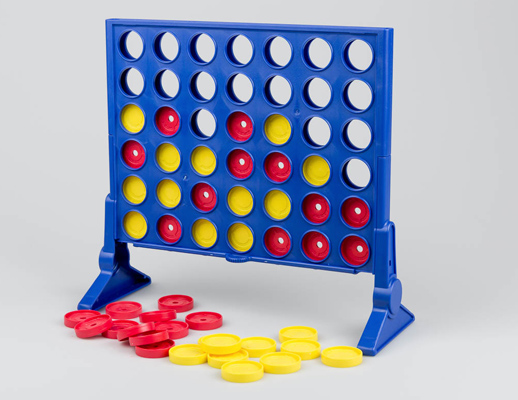
\includegraphics[width=.9\linewidth]{./img/puissance4.jpg}
\end{center}

Dans ce chapitre, tu vas mettre en applications tout ce que tu as appris dans les chapitres précédents. Pour cela, tu vas créer un projet de plus grande envergure que les exercices que tu as faits.

Dans cette section, nous allons créer un \textbf{Puissance 4}. Nous commencerons par le créer à partir des notions que nous avons vues, donc avec une interface en \textbf{ligne de commande}. Par la suite, quand nous étudierons comment créer des interfaces graphiques, nous pourrons revenir sur ce projet pour ajouter des visuels plus intéressants.

\textbf{Les consignes qui sont données dans ce chapitre sont là pour t'aider à réaliser le projet. Le but est que tu développes le Puissance 4 en t'aidant le moins possible des consignes : dans un projet comme celui-ci, il n'y a pas \og une seule bonne réponse\fg{}, chacun peut avoir des idées différentes pour développer et c'est le meilleur moyen de progresser. Si tu es en trop grande difficulté, les étapes décrites dans ce chapitre sont là pour t'aider.}

Si tu as des idées d'améliorations ou que tu veux faire quelque chose différemment, tu es libre de les réaliser, c'est ton projet ! Néanmoins, le professeur vérifiera que ton travail est correct et correspond aux bonnes pratiques de Python que nous avons étudiées.

\subsection*{Règles du Puissance 4}
\label{puissance4_règles}
Le but du jeu est d'aligner une suite de 4 pions de même couleur sur une grille comptant \textbf{6 rangées} et \textbf{7 colonnes}. Chaque joueur dispose de 21 pions d'une couleur, en général jaune ou rouge. Tour à tour, les deux joueurs placent un pion dans la \textbf{colonne} de leur choix, le pion \textbf{coulisse alors jusqu'à la position la plus basse possible dans la dite colonne} à la suite de quoi c'est à l'adversaire de jouer. Le vainqueur est le joueur qui réalise le premier un \textbf{alignement (horizontal, vertical ou diagonal) consécutif d'au moins quatre pions de sa couleur.} Si, alors que toutes les cases de la grille de jeu sont remplies, aucun des deux joueurs n'a réalisé un tel alignement, la partie est déclarée nulle.

\subsection*{Étape 1 : Définir la structure de notre programme}
\label{puissance4_etape1}
Dans cette étape, tu ne vas pas encore coder. Nous allons d'abord réfléchir à la structure de notre programme et imaginer son fonctionnement général. Il faut que l'on définisse de quelles fonctions nous auront besoin pour faire fonctionner notre programme.
Parfois, il est utile d'utiliser du \og pseudo code\fg{}. Le pseudo code, c'est une façon d'écrire un algorithme de façon presque naturelle, sans langage de programmation. Par exemple, dans un pseudo code on peu écrire :
\begin{verbatim}
si (utilisateur écrit "Bonjour") alors
    afficher "Bonjour"
sinon
    afficher "Au revoir"
\end{verbatim}
Le pseudo code aide à déterminer quelles actions notre programme devra effectuer.

Notre programme ne comportera que des fonctions. Chaque action devra être effectuée grâce à une fonction. C'est comme ça que l'on programme : ça permet de pouvoir s'y retrouver plus facilement dans le code et de pouvoir mieux repérer nos erreurs.

La seule instruction qui ne sera pas dans une fonction sera celle qui lance le jeu !

\subsubsection*{Fonctionnement de la grille}
\label{sec:orgc471b5b}
La \og grille\fg{} du jeu sera représentée par une liste \textbf{à deux dimension}, c'est à dire une liste de plusieurs listes. Ce sera donc une liste contenant 6 listes qui contiendront chacune 7 chiffres. Chaque sous-liste de la grille représentera une ligne de la grille. Comme le Puissance 4 contient 7 colonnes, chaque ligne aura donc 7 chiffres. La valeur d'une case de la grille a 3 possibilités :
\begin{itemize}
\item \textbf{0} : la case est libre.
\item \textbf{1} : un jeton du joueur 1 est placé ici.
\item \textbf{2} : un jeton du joueur 2 est placé ici.
\end{itemize}

Au début, la grille sera remplie de \textbf{0} :
\begin{verbatim}
[[0,0,0,0,0,0,0],
 [0,0,0,0,0,0,0],
 [0,0,0,0,0,0,0],
 [0,0,0,0,0,0,0],
 [0,0,0,0,0,0,0],
 [0,0,0,0,0,0,0]]
\end{verbatim}

Lorsqu'un joueur placera un pion, il devra choisir seulement la colonne. À nous de \og simuler\fg{} le fait que le pion tombe jusqu'à la première ligne disponible. Nous aurons une fonction pour cela. Par exemple, si le joueur 1 décide de placer son pion dans la colonne 3 (en partant de 0), la grille contiendra :
\begin{verbatim}
[[0,0,0,0,0,0,0],
 [0,0,0,0,0,0,0],
 [0,0,0,0,0,0,0],
 [0,0,0,0,0,0,0],
 [0,0,0,0,0,0,0],
 [0,0,0,1,0,0,0]]
\end{verbatim}
Si le joueur 2 décide de placer son pion dans la même colonne que le joueur 1, la grille deviendra :
\begin{verbatim}
[[0,0,0,0,0,0,0],
 [0,0,0,0,0,0,0],
 [0,0,0,0,0,0,0],
 [0,0,0,0,0,0,0],
 [0,0,0,2,0,0,0],
 [0,0,0,1,0,0,0]]
\end{verbatim}

Et ainsi de suite.

Par exemple, si les jetons jaunes sont ceux du joueur 1 et les jetons rouges ceux du joueur 2, nous pouvons représenter la grille comme cela :

\begin{center}
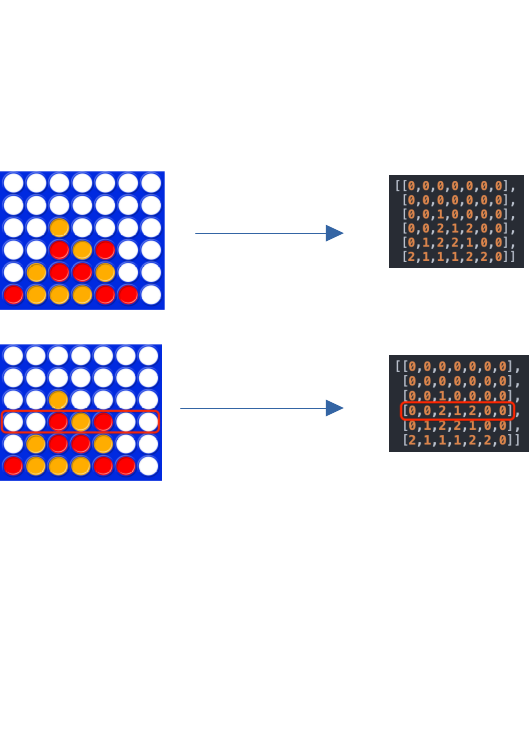
\includegraphics[width=.9\linewidth]{./img/schema_liste.png}
\end{center}

Pour parcourir une liste à deux dimensions, c'est à dire effectuer un test ou une action sur chaque case de la liste, nous utilisons une double boucle. En effet, par exemple si l'on veut ajouter un pion du joueur 1 dans la 2\textsuperscript{ème} colonne de la 3\textsuperscript{ème} ligne, il faut écrire :
\begin{verbatim}
grille[2][1] = 1
# grille[ligne][colonne]
\end{verbatim}

Le premier indice correspond à la ligne et le second à la colonne. Alors pour parcourir et afficher toute la liste :
\begin{verbatim}
for ligne in range(len(grille)):
    for colonne in range(len(grille[ligne])):
        print(grille[ligne][colonne])
\end{verbatim}

\subsubsection*{Liste des fonctions}
\label{sec:orge50fa41}
Maintenant que nous avons une idée générale du fonctionnement de la \textbf{grille de jeu}, voici une liste exhaustive des fonctions dont nous aurons besoin. Tu n'as pas besoin de tout comprendre dès le début, cette section servira aussi plus tard pour t'y retrouver dans toutes les fonctions. Ne commences pas non plus à coder les fonctions ici car nous allons revenir en détail sur chacune d'elles dans les étapes suivantes.

L'important est de visualiser à peu près comment sera notre programme.

\begin{itemize}
\item \texttt{jeu()} : c'est la fonction qui lancera le jeu et le relancera une fois la partie terminée si le joueur en a envie.
\begin{itemize}
\item \texttt{initialiserGrille()} : cette fonction permettra d'initialiser (mettre à zéro) la grille du Puissance 4. C'est comme si elle enlevait les pions ! On utilisera cette fonction avant chaque début de partie, dans la fonction \texttt{jeu()}.
\item \texttt{boucleDeJeu()} : c'est la fonction qui demandera aux joueurs de choisir où poser leurs jetons et les placera tant qu'aucun des deux joueurs n'aura gagné et que la grille n'est pas pleine. Quand le jeu est fini, elle retourne le numéro du joueur qui a gagné (ou \texttt{False} si c'est un match nul).
\begin{itemize}
\item \texttt{joueurGagne(joueur)} : cette fonction détermine si le \texttt{joueur} passé en argument a gagné la partie. Elle sera utilisée dans la fonction \texttt{boucleDejeu()}.
\begin{itemize}
\item \texttt{verifierHorizontalement(joueur)} : vérifie si le joueur passé en paramètre a aligné 4 pions horizontalement dans la grille. Elle sera utilisée dans la fonction \texttt{joueurGagne(joueur)}.
\item \texttt{verifierVerticalement(joueur)} : vérifie si le joueur passé en paramètre a aligné 4 pions verticalement dans la grille. Elle sera utilisée dans la fonction \texttt{joueurGagne(joueur)}.
\item \texttt{verifierDiagonale(joueur)} : vérifie si le joueur passé en paramètre a aligné 4 pions en diagonale dans la grille. Elle sera utilisée dans la fonction \texttt{joueurGagne(joueur)}.
\end{itemize}
\item \texttt{verifierGrillePleine()} : cette fonction devra parcourir la grille pour vérifier s'il y a encore de la place pour poser des jetons.
Elle sera utilisée dans la fonction \texttt{boucleDeJeu()}.
\item \texttt{afficherGrille()} : cette fonction affiche la grille actuelle. Nous formaterons la grille pour qu'elle apparaisse de manière compréhensible aux joueurs.
Elle sera utilisée dans la fonction \texttt{boucleDeJeu()}
\item \texttt{jouerLeTour(joueurActuel)} : cette fonction demandera à un joueur dans quelle colonne il veut placer son jeton. Elle placera ensuite le jeton au bon endroit, c'est-à-dire à la dernière ligne disponible de la colonne demandée.
Elle sera utilisée dans la fonction \texttt{boucleDeJeu()}
\begin{itemize}
\item \texttt{demanderColonne(joueur)} : cette fonction permet de demander au joueur dans quelle colonne il veut placer son pion. Elle renverra le numéro de la colonne demandée. Elle sera utilisée dans la fonction \texttt{remplirGrille(joueurActuel)}.
\item \texttt{ligneLibreDeLaColonne(colonne)} : cette fonction renverra le numéro de la ligne libre de la colonne choisie par le joueur. Elle sera utilisée dans la fonction \texttt{remplirGrille(joueurActuel)}.
\item \texttt{placerJeton(joueur, coordonnees)} : cette fonction permet de placer le jeton du \texttt{joueur} passé en paramètre à l'endroit de la grille indiqué par \texttt{coordonnees}. \texttt{coordonnees} sera un tuple qui aura cette forme : \texttt{(ligne, colonne)}. Elle sera utilisée dans la fonction \texttt{remplirGrille(joueurActuel)}.
\end{itemize}
\item \texttt{recupererSymbole(numeroJoueur)} : cette fonction retourne simplement le symbole correspondant au numéro du joueur passé en paramètre. Si le numéro n'est ni 1 ni 2 alors la fonction renverra un espace \textbf{' '}. Par exemple, si nous utilisons 'X' pour le joueur 1 et 'O' pour le joueur 2, la fonction \texttt{recupererSymbole(1)} renverra \textbf{'X'}.
\end{itemize}
\item \texttt{afficherFinDePartie(gagnant)} : cette fonction fera l'affichage de la fin du jeu en félicitant le gagant s'il y en a un et en disant qu'il y a match nul sinon.
\item \texttt{demanderRejouer()} : cette fonction demandera aux joueurs s'ils veulent rejouer et retourne True ou False en fonction de leur réponse.
\end{itemize}
\end{itemize}

\subsection*{Étape 2 : Définir les variables globales}
\label{puissance4_etape2}
Une \textbf{variable globale} est une variable qui pourra être utilisée dans toutes les fontions d'un programme, sans avoir besoin de la passer en paramètre. Pour le Puissance 4, nous aurons besoin de 3 variables. Elles correspondront à \textbf{la grille de jeu}, au \textbf{symbole du joueur 1} et au \textbf{symbole du joueur 2} dans la grille.

Comme vu précédemment, \textbf{La grille} sera une liste de 6 listes qui contiendront chacune 7 chiffres. Chaque sous-liste de la grille représentera une ligne de la grille.

Pour les symboles, je te conseille d'utiliser les caractères \textbf{'X'} et \textbf{'O'} pour bien différencier les joueurs.

Pour créer des variables globales, c'est très simple : c'est comme des variables normales, sauf qu'elles ne sont pas dans une fonction. Pour notre cas, nous appelerons nos variables \texttt{grille}, \texttt{symboleJoueur1} et \texttt{symboleJoueur2} :
\begin{verbatim}
grille = [[0,0,0,0,0,0,0],
          [0,0,0,0,0,0,0],
          [0,0,0,0,0,0,0],
          [0,0,0,0,0,0,0],
          [0,0,0,0,0,0,0],
          [0,0,0,0,0,0,0]]
symboleJoueur1 = 'X'
symboleJoueur2 = 'O'
\end{verbatim}

Nous n'aurons pas besoin d'autres variables globales pour le moment.

\subsection*{Étape 3 : Définir les fonctions d'affichage}
\label{puissance4_etape3}
\subsubsection*{Affichage des symboles des joueurs}
\label{sec:orgea09501}
\begin{itemize}
\item Crée une fonction \texttt{recupererSymbole(numeroJoueur)}. La logique de cette fonction sera :
\begin{verbatim}
si numeroJoueur est égal à 1:
    renvoyer symboleJoueur1
sinon si numeroJoueur est égal à 2:
    renvoyer symboleJoueur2
sinon
    renvoyer le caractère 'espace'
\end{verbatim}
\end{itemize}

\subsubsection*{Affichage de la grille}
\label{sec:orgee830a9}
\begin{itemize}
\item Crée une fonction \texttt{initialiserGrille()} qui utilisera la variable globale \texttt{grille} pour lui redonner sa valeur par défaut :
\begin{verbatim}
global grille
grille = [[0,0,0,0,0,0,0],
          [0,0,0,0,0,0,0],
          [0,0,0,0,0,0,0],
          [0,0,0,0,0,0,0],
          [0,0,0,0,0,0,0],
          [0,0,0,0,0,0,0]]
\end{verbatim}

\item Crée une fonction \texttt{afficherGrille()}. Cette fonction doit simplement afficher toutes les cases de la grille \texttt{grille} (variable globale) pour que ce soit compréhensible pour les joueurs. Il faudra pour cela utiliser une double boucle pour parcourir chaque \og case\fg{} de la liste. Pour chaque case, on doit afficher le symbole correspondant au pion du joueur placé. Dans notre cas, si c'est 1 il faudra afficher 'X'.
Ensuite on peut ajouter des caractères pour bien séparer chaque case. \textbf{Voici un exemple d'affichage} :
\end{itemize}

Début de partie :

\begin{center}
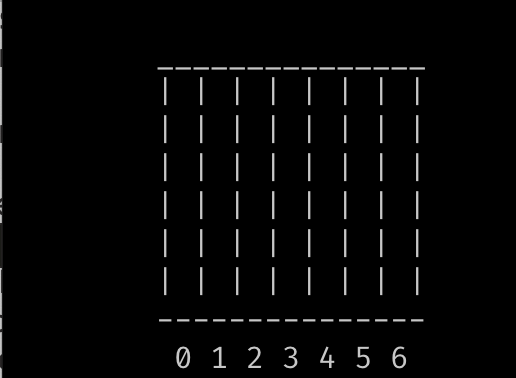
\includegraphics[width=.9\linewidth]{./img/exemple_vide.png}
\end{center}

Après quelques tours :

\begin{center}
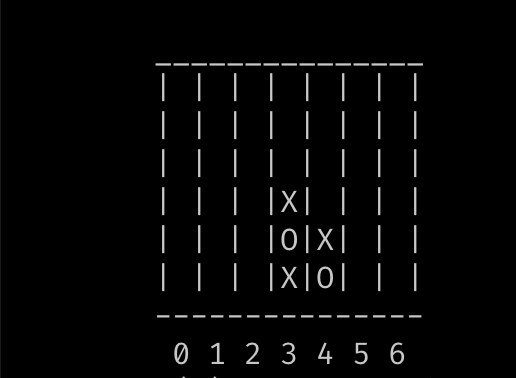
\includegraphics[width=.9\linewidth]{./img/exemple_tours.png}
\end{center}

\subsubsection*{Affichage de fin de partie}
\label{sec:org8f4a80c}
\begin{itemize}
\item Crée une fonction \texttt{afficherFinDePartie} qui prend en paramètre une variable \texttt{gagnant}. Cette fonction doit :
\begin{itemize}
\item Afficher la grille.
\item Afficher un texte qui dit quel joueur a gagné. Dans le cas où c'est un match nul, \texttt{gagnant} aura comme valeur \textbf{0}. Ne pas oublier ce cas-là !
\end{itemize}
\end{itemize}

\textbf{Tu peux tester tes fonctions d'affichage en les appelant dans le programme, pour être sûr que ce qui est affiché correspond bien à ce que tu voulais.}

\subsection*{Étape 4 : Définir les fonctions pour lancer le jeu}
\label{puissance4_etape4}
\begin{itemize}
\item Crée une fonction \texttt{boucleDeJeu()} qui contiendra seulement le mot clef \texttt{pass}. Nous coderons cette fonction à l'étape suivante mais nous avons besoin de l'appeler dans la fonction de lancement du jeu.
\begin{verbatim}
def boucleDeJeu():
    pass
\end{verbatim}

\item Crée une fonction \texttt{demanderRejouer()}. Elle devra :
\begin{itemize}
\item Demander à l'utilisateur s'il veut rejouer tant que sa réponse n'est ni 'o' ni 'n'. Il devra taper 'o' s'il veut rejouer et 'n' s'il veut arrêter.
\item Retourner True si l'utilisateur veut rejouer et False sinon.
\end{itemize}

\item Crée une fonction \texttt{jeu()} :
\begin{itemize}
\item Tant que l'utilisateur veut rejouer, il faut :
\begin{itemize}
\item Initialiser la grille en utilisant la fonction adéquate.
\item Appeler la fonction \texttt{boucleDeJeu()} et recuperer son resultat.
\item Afficher le message de fin de partie en utlisant la fonction adéquate.
\item Demander à l'utilisateur s'il veut rejouer en utilisant la fonction adéquate.
\end{itemize}
\item Quand on sort de la boucle, cela veut dire que l'utilisateur ne veut plus jouer. Dans ce cas, il faudra juste afficher \og Au revoir !\fg{}.
\end{itemize}
\end{itemize}

\subsection*{Étape 5 : Déroulement d'une partie}
\label{puissance4_etape5}
Dans cette étape nous allons commencer la fonction principale \texttt{boucleDeJeu()}. Nous allons préparer la logique et nous coderons les fonctions intérmédiaires au fur et à mesure des étapes suivantes.

\subsubsection*{Fonctions intermédiaires}
\label{sec:org5944326}
Pour commencer, nous allons déclarer les fonctions utilisées dans \texttt{boucleDeJeu()} sans pour autant en écrire le code, avec le mot-clef \texttt{pass} :
\begin{itemize}
\item Crée une fonction \texttt{joueurGagne()} qui prend en paramètre \texttt{joueur}.
\item Crée une fonction \texttt{verifierGrillePleine()}.
\item Crée une fonction \texttt{jouerLeTour()} qui prend en paramètre \texttt{joueur}.
\end{itemize}

\subsubsection*{Boucle du jeu}
\label{sec:org9aee9db}
Définissons maintenant la logique de la boucle de jeu :
\begin{itemize}
\item Modifie la fonction \texttt{boucleDeJeu()} en enlevant l'instruction \texttt{pass}
\item Nous avons besoin d'une variable qui contiendra le numéro du joueur qui doit jouer. Cette variable sera toujours égale à 1 au début d'un partie (le joueur 1 commence).
\item Tant que la grille n'est pas pleine (\texttt{verifierGrillePleine()}), il faut :
\begin{itemize}
\item Afficher la grille.
\item Jouer le tour du joueur actuel (sans oublier de préciser quel joueur).
\item Si le joueur actuel gagne (\texttt{joueurGagne(...)}), il faut renvoyer la valeur du joueur gagnant.
\item Sinon, inverser le numéro du joueur (la variable devient 2 si on fait jouer 1 et vice-versa).
\end{itemize}
\item Quand c'est fini, cela signifie qu'il y a match nul. Dans ce cas, il faudra renvoyer \textbf{0}.
\end{itemize}

\subsection*{Étape 6 : Déroulement d'un tour}
\label{puissance4_etape6}
Nous allons maintenant coder le déroulement d'un tour. Voici ce qu'il se passe à chaque tour :
\begin{itemize}
\item On demande à un joueur de choisir la colonne où placer son jeton. On lui redemande tant qu'il choisi une colonne inexistante (<0 ou >6).
\item On trouve quelle ligne est la première ligne libre (en partant du bas) de la colonne choisie.
\item On place le jeton du joueur dans la grille, aux coordonnées ainsi trouvées.
\end{itemize}

\subsubsection*{Demander la colonne}
\label{sec:org3fa3f26}
Commençons par la fonction qui demande la colonne au joueur :
\begin{itemize}
\item Crée une fonction \texttt{demanderColonne()} qui prend en paramètre \texttt{joueur}. Cette fonction doit :
\begin{itemize}
\item Afficher un message demandant au joueur de choisir sa colonne (préciser à quel joueur on demande pour que ce soit plus clair).
\item Récupérer son choix et le convertir en entier.
\item Recommencer tant que le choix de colonne est incorrect (afficher un message précisant pourquoi on redemande au joueur un numéro de colonne).
\item Retourner le choix de l'utilisateur.
\end{itemize}
\end{itemize}

\subsubsection*{Trouver la ligne où placer le jeton}
\label{sec:org02566a3}
Passons maintenant à la fonction qui trouve la ligne libre d'une colonne. Nous allons devoir coder une fonction qui parcourt chaque ligne de la grille pour vérifier si la colonne choisie est libre sur cette ligne. (Voir le fonctionnement de la grille à l'étape 1 pour savoir si une case est libre).

Il faudra garder la dernière ligne libre trouvée, car le parcours de la liste se fait de haut en bas et que nous devons placer les jetons le plus bas possible.
\begin{itemize}
\item Crée une fonction \texttt{ligneLibreDeLaColonne()} qui prend en paramètre la \texttt{colonne}. Cette fonction doit parcourir toutes les lignes de la \texttt{colonne} afin de trouver la colonne libre la plus basse. Elle devra renvoyer le numéro de la ligne libre et -1 si aucune ligne n'est libre pour cette \texttt{colonne}.
\end{itemize}

\subsubsection*{Placer le jeton}
\label{sec:org8c6619a}
La dernière fonction intermédiaire pour un tour sera la fonction \texttt{placerJeton(joueur, coordonnees)}. Cette fonction placera simplement le numéro du \texttt{joueur} à un l'endroit défini par le tuple \texttt{coordonnees}.

\subsubsection*{Jouer le tour}
\label{sec:org587f6f8}
Enfin, nous allons pouvoir créer la fonction qui fait jouer le tour au joueur :
\begin{itemize}
\item Modifie la fonction \texttt{jouerLeTour()} précédemment créée en supprimant le mot-clef \texttt{pass}. Voici la logique de la fonction :
\begin{itemize}
\item Tant que la \texttt{ligne} vaut \textbf{-1} (c'est à dire est incorrecte) :
\begin{itemize}
\item Demander la colonne au joueur (récupérer le résultat).
\item Trouver la ligne libre pour cette colonne (récupérer le résultat).
\item Si la ligne vaut encore \textbf{-1} dire au joueur que la colonne qu'il a choisie n'est plus libre.
\end{itemize}
\item Quand on a trouvé la ligne correspondant à la colonne choisie, placer le jeton du joueur aux coordonnées trouvées.
\end{itemize}
\end{itemize}

Nous avons fini de créer le déroulement d'un tour. Dans la prochaine étape, nous nous attaquerons à la fonction qui trouve le gagnant d'une partie.

\subsection*{Étape 7 : Y a-t-il un vainqueur ?}
\label{puissance4_etape7}
Désormais, on peut faire jouer un tour à un joueur. Il faut maintenant que l'on puisse déterminer à chaque fin de tour si le joueur qui vient de jouer a gagné ou s'il y a match nul.

Pour cela, nous utiliserons deux fonctions différentes : une première qui permet de vérifier si un joueur passé en paramètre a gagné et une seconde qui permet de vérifier si la grille est pleine.

\subsubsection*{Trouver un alignement}
\label{sec:orgef45479}
Nous allons commencer par déterminer si un joueur a gagné. Pour cela, nous devons créer 3 fonctions intermédiaires :
\begin{itemize}
\item \texttt{verifierHorizontalement(joueur)} : cette fonction vérifie si le joueur spécifié passé en paramètre a un \textbf{alignement horizontal} de 4 jetons. Pour cela, il faut parcourir toutes les lignes de la liste pour vérifier si le numéro du joueur apparaît 4 fois de suite dans la ligne.
\item \texttt{verifierVerticalement(joueur)} : cette fonction vérifie si le joueur spécifié a un \textbf{alignement vertical} de 4 jetons. Il faudra parcourir chaque colonne de la liste pour vérifier si le numéro du joueur apparaît 4 fois de suite dans la colonne. \textbf{Conseil} : pas besoin de commencer la vérification au-delà de la 3\textsuperscript{ème} ligne, car ce n'est plus possible d'aligner 4 pions sur 3 lignes !
\item \texttt{verifierDiagonale(joueur)} : cette fonction vérifie si le joueur spécifié a un \textbf{aligement en diagonale} de 4 jetons. Il faudra parcourir toute la liste en cherchant si le numéro du joueur apparaît 4 fois de suite dans une diagonale \textbf{ou dans l'autre}. En effet, n'oublie pas les deux sens possibles d'une diagonale ! Cette fonction sera un peu plus difficile que les autres, je te conseille de commencer par essayer de parcourir les diagonales de la liste en faisant des tests d'affichage.
\end{itemize}

\subsubsection*{Le joueur a-t-il a gagné ?}
\label{sec:orgc19f46e}
Maintenant que nous avons codé nos 3 fonctions intermédiaires, nous pouvons modier la fonction \texttt{joueurGagne(joueur)}. La fonction doit maintenant renvoyer \texttt{True} si le \texttt{joueur} a un alignement horizontal, vertical ou en diagonale. Sinon, elle retourne \texttt{False}.

\subsubsection*{Match nul ?}
\label{sec:org79ab8df}
Enfin, il nous manque la fonction qui vérifie s'il y a \textbf{match nul}. Nous savons qu'il y a match nul si la grille est remplie et que personne n'a gagné. Alors, nous avons simplement besoin d'une fonction qui vérifie si la grille est pleine :
\begin{itemize}
\item Modifie la fonction \texttt{verifierGrillePleine()}. Elle doit renvoyer \texttt{True} si la grille est pleine et \texttt{False} sinon.
\end{itemize}

\subsection*{Étape 8 : Lancement du jeu !}
\label{puissance4_etape8}
Désormais, il ne nous reste plus qu'à lancer le jeu : appelle simplement la fonction \texttt{jeu()} dans le programme !

Quand tu vas tester le jeu, il est très fort probable qu'il y ait des \og bugs\fg{} et que certaines choses ne fonctionnent pas : c'est normal pour un gros programme. Ne t'inquiètes pas et n'hésite pas à faire plein de tests pour chaque fonction pour trouver d'où vient le problème.


\section*{Intelligence Artificielle du Puissance 4}
\label{ia_puissance4}
\subsection*{Théorie}
\label{ia_puissance4_theorie}
\subsubsection*{Ressources}
\label{sec:orgf6f81cc}
\url{https://www.youtube.com/watch?v=0lQxdR6IqCA\&t=103s}

Un cours de fac plutôt bien résumé : \href{./manuel/Minmax.pdf}{MinMax}

\subsection*{Code}
\label{ia_puissance4_code}
\subsubsection*{Étape 1 : Tous les coups possibles}
\label{sec:orgaa85888}
Crée une fonction qui doit retourner la liste de tous les coups possibles au prochain tour. Chaque élément de la liste sera un tuple correspondant à la ligne et la colonne où le jeton peut être placé : \textbf{(ligne, colonne)}.

\subsubsection*{Étape 2 : Tous les alignements}
\label{sec:org67aefe5}
Crée une fonction qui retourne la liste de tous les alignements de 4 cases de la grille. La liste contiendra donc des listes de 4 éléments. Les alignements possibles sont :
\begin{itemize}
\item En ligne
\item En colonne
\item En diagonale vers la droite
\item En diagonale vers la gauche
\end{itemize}

\subsubsection*{Étape 3 : Fonction d'évaluation}
\label{sec:org1b8610b}
Crée une fonction qui devra attribuer un \og score\fg{} à une grille pour un joueur donné. Cette fonction permettra à l'IA de savoir quel coup lui rapporte le plus de points. Elle sera utilisée plus tard dans la fonction chargée d'anticiper quel coup amènera au meilleur résultat.
Voici quelques indications :

Le score varie en fonction des alignements de 4 encore possibles pour le joueur donné en paramètres. C'est ici que tu auras besoin de la fonction de l'étape 2. Sers-toi de la liste pour parcourir chaque alignement et vérifier si le joueur en paramètre peut encore aligner 4 pions dedans.

S'il peut, alors il faut compter combien de pions sont déjà présents dans l'alignement. Si c'est l'autre joueur qui peut, il faut aussi sauvegarder son score dans une autre variable. Attention, il ne faut pas ajouter 1,2 ou 3 au score car dans ce cas on ne peut pas savoir si 3 correspond à 3 pions alignés ou 3 pions dans 3 alignements différents. Pour contrer ce problème, voici la grille du score à ajouter en fonction du nombre de pions alignés :

\begin{center}
\begin{tabular}{rr}
Pions alignés & Score \\[0pt]
\hline
0 & +0\\[0pt]
1 & +1\\[0pt]
2 & +100\\[0pt]
3 & +10000\\[0pt]
4 & +1000000\\[0pt]
\end{tabular}
\end{center}

Quand les scores des deux joueurs ont été calculés, la fonction devra renvoyer le score du joueur en paramètre moins le score de l'adversaire.

\subsection*{Un peu de cours}
\label{sec:org1effec5}
\subsubsection*{Recherche}
\label{sec:org5e9c9da}
Le jeu du Puissance 4 est un jeu dit \textbf{déterministe} et \textbf{complètement observable}. Cela siginifie que l'agent sait dans quel état il est et dans quel état il sera (en fonction des actions qu'il fait). La solution de ce type de problème est une suite d'actions (par exemple \og jouer dans la colonne n°3\fg{}).

Pour trouver la meilleure solution possible dans un état donné, l'agent doit connaître toutes les possibilités de jeu et leurs conséquences. Nous utilisons pour imager cela un \textbf{arbre de recherche}. Cet arbre de recherche permet de parcourir toutes les possibilités de jeu.

Exemple de l'arbre de recherche du morpion (ou tic-tac-toe) :

\begin{center}
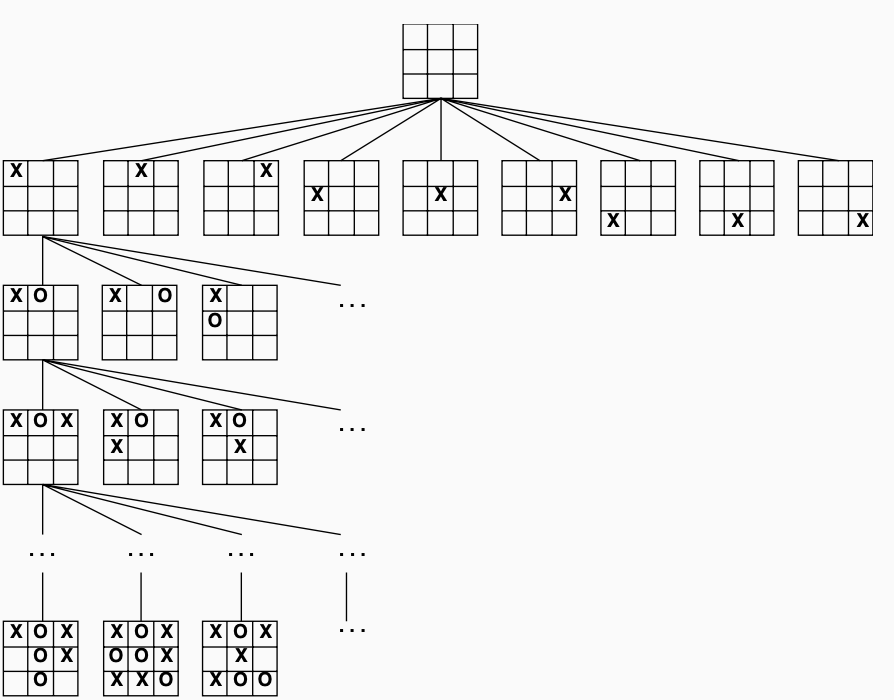
\includegraphics[width=.9\linewidth]{./img/arbre-recherche.png}
\end{center}

Pour pouvoir générer cet arbre de recherche pour notre IA, nous avons créé une fonction qui retourne tous les coups possibles, c'est-à-dire tous les ensembles \texttt{(ligne, colonne)} correspondants aux endroits où le prochain joueur peut placer son pion.

\subsubsection*{Algorithme Min-Max}
\label{sec:orgb22c829}
L'algorithme Min-Max est un algorithme utilisé uniquement pour la programmation d'intelligences artificielles de jeux. Le principe est le suivant:
\begin{itemize}
\item Quand c'est au tour de l'agent de jouer (notre IA), il doit trouver la solution qui lui offrira le plus de chances de gagner. Pour ce faire, il va devoir \textbf{tester tous les coups} qu'il peut jouer dans l'\textbf{état actuel} de la grille.
\item Pour chaque coup possible, il vérifie le résultat (a-t-il gagné ?) et va tester \textbf{tous les coups que l'adversaire pourra jouer ensuite}.
\item L'agent continue de \og simuler\fg{} la partie jusqu'à ce qu'il arrive dans un \textbf{état final}, c'est-à-dire un état où soit un des joueurs a gagné soit la grille est remplie.
\item L'agent doit recommencer cette simulation de partie pour tous les coups possibles à chaque fois.
\end{itemize}

C'est ici que nous aurons besoin d'utiliser la récursion : l'agent devra tester toutes les parties possibles pour déterminer quel coup amène la partie vers sa victoire. Chaque \og étape\fg{} ou \og étage\fg{} dans l'arbre de recherche correspond à ce que l'on appelle \textbf{la profondeur}. Plus l'agent va en profondeur, plus le temps de recherche sera long car à chaque prondeur, cela ajoute encore plus de solutions à vérifier.

\textbf{L'algorithme Min-Max est donc une manière de générer et explorer l'arbre de recherche associé à la partie de Puissance 4.}

Le fonctionnement de l'algorithme est le suivant :
\begin{itemize}
\item Max et Min sont les deux joueurs.
\item Max joue en premier, Min en second.
\item Le joueur Max (qui correspond à l'agent) cherche à obtenir le score maximal avec son coup.
\item Le joueur Min (qui correspond au joueur humain) cherche à obtenir le score minimal avec son coup.
\end{itemize}

Le Puissance 4 est un \textbf{jeu à somme nulle}. Nous pouvons traduire cela par le fait que :
\begin{itemize}
\item Quand le joueur 1 gagne, le joueur 2 a perdu.
\item Quand le joueur 2 gagne, le joueur 1 a perdu.
\item Quand il y a match nul, aucun des joueurs n'a gagné.
\end{itemize}
Nous avons déjà pu remarquer ça quand nous avons programmé les fonctions pour déterminer le vainqueur d'une partie : quand on trouve l'alignement d'un joueur, nous n'avons plus besoin de vérifier le reste de la grille.

\textbf{Pour l'algorithme Min-Max, nous aurons donc trois \og scores\fg{} possibles pour une grille} :
\begin{itemize}
\item 1 si Max gagne.
\item -1 si Min gagne.
\item 0 si aucun des deux ne gagne.
\end{itemize}

Le pseudo-code de l'algorithme Min-Max se trouve à la page 12 du cours dans la partie \textbf{Ressources}.

\subsection*{Retour au code}
\label{sec:org0bbb02e}
Pour notre jeu, nous utiliserons deux fonctions : \texttt{min\_max(joueur\_max, is\_tour\_max, profondeur)} et \texttt{trouver\_meilleur\_coup(joueur\_max, profondeur)}.

\begin{itemize}
\item La fonction \texttt{trouver\_meilleur\_coup(...)} doit :
\begin{itemize}
\item Récupérer tous les coups possibles.
\item Initialiser \texttt{meilleur\_score} à \texttt{-math.inf}.
\item Initialiser \texttt{meilleur\_coup} à \texttt{None}.
\item Pour chaque coup possible :
\begin{itemize}
\item Placer le jeton dans la grille aux coordonnées du coup.
\item Récupérer le score du coup grâce à \texttt{min\_max}.
\item Effacer le coup dans la grille.
\item Garder en mémoire le meilleur score et le meilleur coup.
\end{itemize}
\item Il faudra retourner à la fin les coordonnées du meilleur coup trouvé.
\end{itemize}

\item Pour la fonction \texttt{min\_max(...)}, nous pouvons utiliser le pseudo-code en page 12 du cours dans \textbf{Ressources}.
\end{itemize}
\end{document}